\dictum{
We gather main results and techniques from the formal approach to PDE theory with the focus lying in particular on the construction of power series solutions to a given PDE. These techniques allow us to formulate a second and final requirement that is posed on the gravitational dynamics if spacetime is additionally inhabited by a matter field: the causal compatibility between matter and gravitational EOM. Thus PDE theory bridges the gap between gravitational and matter dynamics.
Moreover, we develop a concise framework for the perturbative computation of gravitational Lagrangians that we formulate in terms of an explicit perturbative construction algorithm.
}
\section{Formal PDE Theory, Symbols and Involution}
Given the achievement of translating the first requirement we wish to pose on any gravitational dynamics --- the invariance under spacetime diffeomorphisms --- into an equivalent linear, first-order PDE system that we presented in the previous chapter, any further considerations that we provide in this chapter aim to solve one of the following two problems:
\begin{itemize}
    \item Assume we are given a concrete matter theory that employs a certain tensor field as background geometry.
    Such a matter theory could, for instance, be phenomenologically motivated. As we do not want to specify the values of the tensorial background geometry by hand we pursue the goal of supplementing the matter theory with dynamical equations that allow us to predict values of the tensor field, i.e., we complete the matter theory with an appropriate theory of gravity for the tensorial geometry. To that end, we try to solve the equivariance equations (\ref{DiffeoEqn}) specifically for the given tensor field. 
    Once we have solved the stated PDE system, we obtain a gravitational Lagrangian that describes the dynamics of this tensor field. The gravitational dynamics is however not independent of the matter field, as the latter will appear as source term in the gravitational EOM, describing how gravity is generated.
    The matter and gravity EOM actually constitute a coupled system (see Figure \ref{MatterGrav}), neither of the EOM can be solved independently. This raises the question of how we can ensure the two theories are, in fact, compatible in the sense that the given EOMs can be solved together.
    \item The above consideration obviously requires that we are able to obtain solutions to the equivariance PDE. This itself in no way constitutes a simple task and certainly demands specific techniques.
\end{itemize}
Although these two problems at first glance seem to have not much in common, it turns out that the key to the solution of either one of them lies in an in-depth treatment of partial differential equations. 
To that end, we will develop some additional tools and techniques that are indispensable for the  \textit{\textbf{formal theory}} PDEs.

\begin{figure}[hbt!]
\centering 
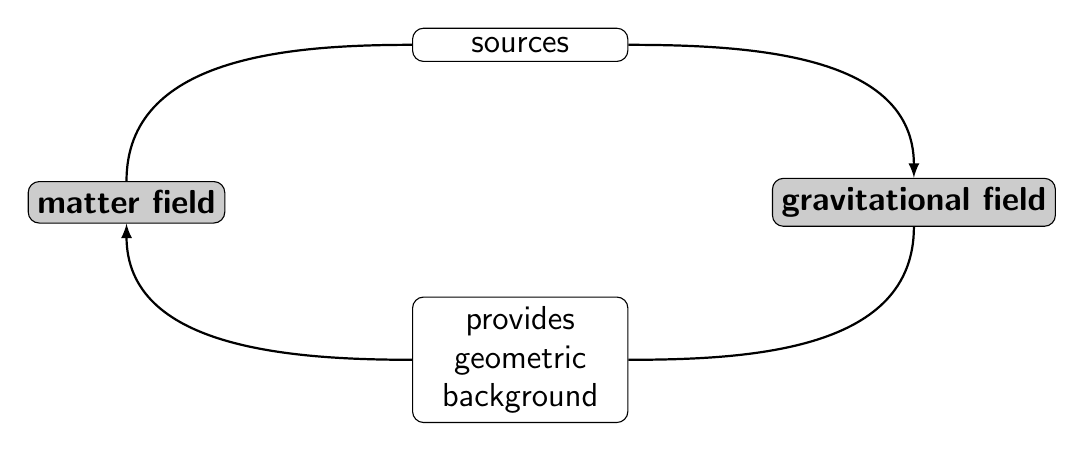
\begin{tikzpicture}[main node/.style={shape=rectangle, rounded corners,draw,fill=gray!40,font=\sffamily\large\bfseries}, side node/.style = {shape=rectangle, rounded corners,draw, font = \sffamily\large, text width = 2.5cm, align = center}]
\node[main node] (M) at (0,0) {matter field};
\node[main node] (G) at (10,0) {gravitational field};
\node[side node] (S) at (5,2) {sources};
\node[side node] (B) at (5,-2) {provides \ \  geometric
background};
\draw [thick] (M) to [out = 90, in = 180] (S);
\draw [-latex, thick] (S) to [out = 0, in = 90] (G);
\draw [thick] (G) to [out = 270, in = 0] (B);
\draw [-latex, thick] (B) to [out = 180, in = 270] (M);
\end{tikzpicture}
\caption{Matter Gravity Coupling}\label{MatterGrav}
\end{figure}

The formal theory of partial differential equations is phrased in terms of differential geometry. A PDE is defined as a submanifold of a jet bundle that is constructed over the bundle with base space coordinates being provided by the \textit{\textbf{independent variables}} and fiber coordinates given by the \textit{\textbf{dependent variables}} of the given problem. The advantage of such a description of partial differential equations does not only lie in the fact that one works now with coordinate independent geometric objects, but the jet bundle approach also enables one to treat the derivatives of a given function as algebraically independent new variables. Thus many problems that arise in the context of PDEs can be stated and solved in terms of basic \textit{\textbf{linear algebra}}. This, in particular yields the additional convenience that many of those arising problems can be tackled by using \textbf{\textit{computer algebra}}.

An introduction to the formal theory of partial differential equations can be found in \cite{saunders_1989}. A comprehensive treatment is provided in \cite{seiler2009involution} were also deeper results regarding the algebraic and homological aspects of the formal PDE theory are included. We will especially follow along the lines of \cite{seiler1994analysis} as there the relevant notions are concisely described with just the right level of rigor that is necessary for our subsequent developments. We start by stating the needed definitions, most of which can be found in \cite{seiler1994analysis}.
\begin{definition}[PDE]
Let $(F,\pi_F,M)$ be a bundle and $J^qF$ the $q$th-order jet bundle over $F$. A $q$th-order PDE $R_q$ on $F$ is a  submanifold of $J^qF$. A solution to a given PDE is a section $G \in \Gamma(F)$ s.t. the jet prolongation $j^q(G)$ lies entirely in $R_q$.  
\end{definition}
Sometimes one additionally requires $R_q$ to be fibered. Thereby one ensures that the PDE poses no restrictions on the independent variables, i.e., the base space coordinates on $M$ (this version is for instance used in \cite{seiler1994analysis}).
For many of the following computations, it is crucial to know the dimension of the jet bundle of order $q$ over a bundle $F$ with base space dimension $m$ and fiber dimension $n$:
\begin{align}
    \mathrm{dim}J^qF = n\binom{m+q}{q}
\end{align}
From this definition of a PDE one can obtain a PDE in the traditional sense by specifying an additional vector bundle $(E,\pi_E,M)$ over the same base space together with a bundle morphism:
\begin{align}
    \begin{aligned}
    \Phi : J^qF &\longrightarrow E\\
    (x^a, v_A, v_{Ap},...,v_{AI_q}) &\longmapsto \Phi^{\tilde{B}}(x^a, v_A, v_{Ap},...v_{AI_q}),
    \end{aligned}
\end{align}
such that the PDE is given as kernel of $\Phi$, i.e.
the PDE is described by the individual component  equations:
\begin{align}
    \Phi^{\tilde{B}}(x^a, v_A, v_{Ap},...v_{AI_q}) = 0.
\end{align}
Whenever we will work with such a representation of a PDE, w.l.o.g. we will always assume that the bundle morphism $\Phi^{\tilde{B}}$ is specified such that the individual component equations are really independent, i.e., the bundle morphism is non-degenerate. 

Given such a representation of a PDE, we can apply the usual jet bundle operations to the individual component functions $\Phi^{\tilde{B}}$, i.e., we can \textit{\textbf{prolong}} them to higher derivative orders by taking the previously defined \textit{\textbf{total derivative}} of the representation $\Phi^{\tilde{B}}$ along any base space direction and we can use the jet bundle projections to \textit{\textbf{project}} them to any lower derivative order at wish. We denote the PDE that is described by the combined set of the given equations $\Phi^{\tilde{B}}=0$ and all possible prolongations $D_i\Phi^{\tilde{B}}=0$ by $R_{q+1} \subset J^{q+1}F$. Similarly we denote higher prolongations of a PDE by $R_{q+r}$. We call $R_{q+r}$ the \textit{\textbf{prolongation}} of $R_q$ to $(q+r)$th-order or short the $r$th prolongation of $R_q$. 

Considering this, it is particularly interesting to first prolong a given PDE and then use the jet projections to define $R_q^{(1)} := \pi_{(q+1),q}\left ( R_{q+1} \right ) \subset J^qF $. As the following example taken from \cite{seiler1994analysis} illustrates this in general does not recover the original equation but only a subset $R_q^{(1)} \subset R_q$, i.e., prolonging and projecting might reveal additional equations.
\begin{example}\label{ExamplePDE}
Consider the PDE on the first-order jet bundle over the trivial bundle $\mathbb{R}^3 \times \mathbb{R}$ with jet bundle  coordinates $(x,y,z,u,u_x,u_y,u_z)$ defined by: 
\begin{align}
    R_1 : \begin{cases} u_z + y \cdot u_x &= 0 \\
                        u_y &= 0.
            \end{cases}
\end{align}
prolonging the first equation w.r.t. $y$, i.e., applying the total derivative: 
\begin{align}
D_y = \partial_y + u_{xy} \cdot \partial_{u_x} + u_{yy} \cdot \partial_{u_y} + u_{yz} \cdot \partial_{u_z}
\end{align}
to it we obtain the equation $u_{yz} + y \cdot u_{xy} + u_x =0$. Prolonging the second equation w.r.t. $x$ and $z$, however, shows that all second-order derivatives in the newly obtained equation vanish and we are left with $u_x = 0$. Inserting this equation into the first equation we furthermore find $u_z = 0$. Hence we find that the prolonged and projected system is given by: 
\begin{align}\label{prolo}
    R_1^{(1)} : \begin{cases} u_x = 0 \\
                        u_y = 0\\
                        u_z = 0 .
            \end{cases}
\end{align}
Note that the involved prolongations were mandatory to get this result; the additional equations in (\ref{prolo})  cannot be obtained by purely algebraic manipulations. 
\end{example}
Such additional independent equations that can only be obtained by prolonging to a higher-order and then projecting the PDE again to the previous order are called \textit{\textbf{integrability conditions}}. 
Usually, they might be found by constructing a specific linear combination of prolonged equations and thereby eliminating appropriate terms that contain derivatives of leading order such that one ends up with an equation of sub-maximal derivative order. In our example, we prolonged the first equation w.r.t. $y$ and then subtracted the prolongation of the second equation w.r.t $x$ and $z$ to discard the second derivatives $u_{xy}$ and $u_{yz}$ respectively. 

If a PDE $R_q$ already contains all its integrability conditions, i.e., if for all $n\geq 0$ it holds that $R_{q+n}^{(1)} = R_{q+n}$ we call it \textit{\textbf{formally integrable}}.
Formal integrability is of particular importance when computing \textbf{\textit{power series solutions}} to a given PDE. The essence of the computation of power series solutions is making a general power series ansatz with arbitrary expansion coefficients for the solution of the PDE and then, by successively inserting the ansatz into the PDE and all necessary prolongations, and evaluating the resulting equations at the expansion point, deriving linear equations for the expansion coefficients. 
To be more precise, we are not interested in computing such solutions up to infinite order and then summing up the series to obtain a real solution of the PDE, but we will simply abort the power series construction after some finite order, neglecting all further contributions that are obtained in higher orders.
If for some reason, the individual contributions are known to decrease with an increase in their order, the aborted power series solution yields a reasonable approximation to the real situation. 
In other words we will consider a \textit{\textbf{perturbative}} treatment of the PDE.
Thus we will only construct the power series ansatz\footnote{Such an ansatz should probably better be called a polynomial ansatz, but to emphasis the similarities to the case of computing real power series solutions we will stick to calling it a (finite) power series ansatz.} up to the desired finite order.

Using adapted coordinates on $F$, such a finite power series solution to a given PDE $R_q$, described by the equations $\Phi^{\tilde{A}} = 0$, can be computed as follows: We take a point $p_0 \in M$ --- in the adapted coordinates on $F$ we define: $x^m(p_0) =: x_0^m$ --- and construct a general section $G\in\Gamma(F)$ as arbitrary, finite power series around $x_0$:
\begin{align}
\begin{aligned}
    G_A(x^m) :=  \sum_{k=0}^{r} a_{AI_k}I^{I_k}_{i_1...i_k}(x^{i_1}-x_0^{i_1}) \cdot ... \cdot (x^{i_k}- x_0^{i_k}), 
\end{aligned}
\end{align}
where $a_{AI_k}$ are constants. Note in particular that the $q$th jet prolongation of $G$ evaluated at $p_0$ then yields, up to combinatorial\footnote{This is a result from our factor-less definition of the finite power series. The factor-less definition is used as it is in closer relation to the later treatment of perturbative Lagrangians.} factors, the following coordinate expression:
\begin{align}
    j^k(G)(p_0) \equiv \left ( x_0^m, a_A, a_{Am}, a_{AI}, ... a_{AI_q} \right ).
\end{align}
Hence plugging in the finite power series into the PDE $\Phi^{\tilde{A}} =0$ and evaluating at $x^m=x^m_0$ yields a purely algebraic equation system for the expansion coefficients up to order $q$, that we can readily solve. Prolonging the equation to order $q+r$ and then plugging in the power series ansatz we obtain algebraic equations for the higher expansion coefficients up to order $q+r$ that feature the priorly solved coefficients $a_{AI_0},...,a_{AI_q}$ as inhomogeneities. We then can solve these equations for the new expansion coefficients $a_{AI_{q+1}}...a_{AI_{q+r}}$. The solutions, in general, will be given by expressions that contain the lower-order coefficients.
The algebraic equation system that we obtain looks as follows:
\begin{align}
\begin{aligned}
R_q &: \Phi^{\tilde{A}}(x_0^m,a_A,...,a_{AI_q}) &&= 0 \\
R_{q+r} &:  D_{J_r}\Phi^{\tilde{A}}(x_0^m,a_A,...,a_{AI_{q+r}}) &&= 0,
\end{aligned}
\end{align}
where as before $D_{J_r} = J^{i_1...i_r}_{J_r} D_{i_1} ... D_{i_r}$.

The occurrence of integrability conditions during prolongations of the PDE then hinders one to construct such a power series solution order by order. Potentially occurring integrability conditions yield further equations for lower-order coefficients that only are present after higher-order prolongations are computed. Thus, once one has solved the problem up to some finite order $r$, it might happen that integrability conditions of higher prolongation order yield additional equations that further restrict the obtained solution. 
Hence the computed solution is, in fact, too general, i.e., it includes fake solutions.
One can, however, in most cases, not easily predict during which prolongations these integrability conditions appear. Therefore, if a PDE is not formally integrable, i.e., if it generates integrability conditions, one can never be sure that obtained perturbative solutions are not too general. To put it differently, one can never be sure if all information that is contained in the PDE is also included in the construction of the power series solution, or if information remains hidden in integrability conditions.

Although the perturbative treatment of PDEs compromises a vast field in theoretical physics, techniques that allow the proof of formal integrability of a given PDE that we will subsequently present, seem to be to a large extent unknown in this area of research. 

Summing up, we have thus seen that the occurrence of integrability conditions thoroughly disturbs the order by order construction of power series solutions. When treating a specific PDE perturbatively, it is, therefore, essential to first check whether or not the PDE is formally integrable; if it is not any obtained solution is practically meaningless.
As we, in particular, want to develop a framework for the perturbative treatment of the equivariance equation (\ref{DiffeoEqn}), we hence have to establish techniques for proofing formal integrability.
Explicitly checking formal integrability of a given PDE is, however, extensively involved, as in principle one would need to probe the infinite number of conditions $R_{q+r}^{(1)} = R_{q+r}$ corresponding to an infinite number of prolongations and projections that one would need to compute. Thus subsequent developments concentrate on how we can predict in advance whether or not integrability conditions occur during specific prolongations of a given PDE, without actually carrying out the explicit computation.

To that end, we take a closer look at a specific step that is involved in  the order by order construction of power series solutions, namely the step of solving the various linear systems.
In each order $q+r$ only a certain number of the newly obtained highest order coefficients $a_{AI_{q+r}}$ is in fact determined by the prolonged PDE $R_{q+r}$, some of the coefficients are not governed by the PDE at all and can hence be chosen freely.
For the particular case of \textit{\textbf{quasilinear}}\footnote{Note that although if $R_q$ is not quasilinear, all its prolongations will be quasilinear as the total derivative always yields quasilinear equations. For the same reason PDEs that are obtained as EOMs to a given Lagrangian will always be quasilinear.} PDEs, i.e., PDEs that are linear in the highest order derivatives that occur, the expansion coefficients that can be chosen freely are given by the kernel of a matrix that is obtained from the highest derivative part of the PDE. This matrix is called the \textit{\textbf{symbol}} of the PDE.
\begin{definition}[symbol]
Given a PDE $R_q$ with representation $\Phi^{\tilde{B}}=0$, its symbol is the following matrix that only contains the highest-derivative-order contributions to $R_q$:
\begin{align}
    M_q : M_q^{(\tilde{B})({AI_q})} := \left ( \frac{\partial \Phi^{\tilde{B}}}{\partial v_{AI_q}} \right ).
\end{align}
The rows of the symbol are labeled by the independent equations $\tilde{B}$, i.e., the components of $(\Phi^{\tilde{B}})$, the columns are labeled the different highest-derivative-order contributions $(AI_q)$.
Similarly we can directly obtain the symbol of the prolonged equations $R_{q+r}$ as:
\begin{align}\label{proSym}
    M_{q+r} : M_{q+r} ^{(\tilde{B}I_r) (AI_{q+r})}:= \left ( \frac{\partial D_{I_r}\Phi^{\tilde{B}
    }}{\partial v_{AI_{q+r}}} \right ). 
\end{align}
Note that now the rows are labeled by order $r$ prolongations of individual equations $(\tilde{B}I_r)$\footnote{As the notation of: $M_{q+r} ^{(\tilde{B}I_r) (AI_{q+r})}$ for the prolonged symbol really only is used to indicate the way we arrange the different contributions in the matrix the reader should not be confused by the appearance of $I_r$ in upper position on the left-hand-side and in lower position on the right-hand-side.}.
\end{definition}
It is important to observe that the symbol of a quasilinear PDE really only collects its highest-derivative-order coefficients in matrix form.
If the PDE $R_q$ contains a contribution proportional to $\frac{\partial \Phi^{\tilde{B}}}{\partial v_{AI_q}}$ , recalling the definition of the total derivative (\ref{totDer}), we find that the prolonged PDE $R_{q+r}$ involves precisely the same contribution, but multiple times and possibly in multiple of its individual equations. 
To be more precise, the matrix components of the prolonged symbol matrix are given by:
\begin{align}
M_{q+r}^{(\tilde{B}I_r) (AI_{q+r})} = 
\begin{cases}
M_q^{(\tilde{B}) (AI_q)}  & \text{if \ \ }  
    v_{AI_{q+r}} = D_{I_r} v_{AI_q} \\
0 & \text{otherwise}.
\end{cases}
\end{align} 
We now use that: 
\begin{align}
    D_{I_r}v_{AI_q} = v_{AI_{q+r}}I_{I_q I_r}^{I_{q+r}}.
\end{align}
Thus we see that we can easily express the prolonged symbol $M_{q+r}$ by the matrix elements of the unprolonged symbol $M_q$ as:
\begin{align}
    \begin{aligned}
    M_{q+r} : M_{q+r} ^{(\tilde{B}I_r) (AI_{q+r})}  = \left ( \frac{\partial \Phi^{\tilde{B}}}{\partial v_{AI_q}} \right ) I_{I_q I_r}^{I_{q+r}} .
    \end{aligned}
\end{align}
We will synonymously call the matrix and the corresponding linear equation system the symbol of the PDE. The precise meaning can be inferred from the context. 


Although only containing contributions from the highest derivative order, the symbol already incorporates considerable amounts of the PDE's overall information.
When constructing order by order power series solutions
a general power series ansatz contains
$n\binom{m+q-1}{m-1}$ undetermined expansion coefficients $a_{AI_q}$ of order $q$th. 
Precisely those expansion coefficients $a_{AI_q}$ that lie in the kernel of the symbol $M_q$ are not restricted by the PDE $R_q$ and thus can be specified arbitrarily. In particular, the number of such arbitrary expansion coefficients equals the dimension of the kernel of $M_q$. 
Hence the rank of the symbol $M_q$ contains the complete information regarding how many undetermined expansion coefficients of order $q$ appear in the general power series solution.
Similarly, the ranks of the prolonged symbols $M_{q+r}$ yield this information for higher-order expansion coefficients $a_{AI_{q+r}}$.

If we restrict attention to analytic solutions of a given PDE, and further disregard questions concerning the convergence of the power series solutions for a moment, then such undetermined expansion coefficients in the general power series solution are in one-to-one correspondence with arbitrary Taylor coefficients in the expansion of the general analytic solution. Thus the symbol $M_q$ and all its prolongations $M_{q+r}$ govern all the information of how many arbitrary Taylor coefficients the general analytic solution of the PDE contains, i.e., these matrices contain the entire information about the size of the formal\footnote{As we disregarded the question of convergence of power series solutions such power series are also called formal power series. } solution space of the given PDE. 

For our future developments, the symbol, however, foremost attains its significance due to its close relation to the occurrence of integrability conditions.
Note that for integrability conditions to occur during a prolongation, it must be possible to form a certain linear combination of prolonged equations that does not contain contributions in the highest derivative order. Such linear combinations only exist if the symbol has sub-maximal rank, i.e., suffers from rank defects, as the specific linear combination of equations that does not contain contributions in highest derivative order then precisely produces a zero-row in the symbol matrix. This can be seen in more detail by prolonging a given PDE and then taken its linearization, i.e., the Jacobi matrix of its representation:
\begin{align}
\def\arraystretch{2.5}
\begin{bmatrix}
      \ \ \mathlarger{{\frac{\partial D_i\Phi^{\tilde{A}}}{\partial v_{AI_{q+1}}}}} \ & \vline & \mathlarger{\frac{\partial D_i \Phi^{\tilde{A}}}{\partial v_{AI_k}}}, \ \ k \leq q \ \  \\
        \cmidrule(lr){1-3}
        \mathlarger{0} & \vline & \mathlarger{\frac{\partial \Phi^{\tilde{A}}}{\partial v_{AI_k}}}, \ \ k \leq q \ \
\end{bmatrix}.
\end{align}
The lower right block is simply the Jacobi matrix of the unprolonged PDE. The upper left block is precisely the prolonged symbol matrix $M_{q+1}$. Only if $M_{q+1}$ has sub-maximal rank there exist certain linear operations that produce zero rows in $M_{q+1}$ and hence yield equations of sub-maximal derivative order. If such linear combinations exist, the prolongation, however, does not necessarily produce integrability conditions.
There exist essentially three possibilities:
\begin{itemize}
    \item If the corresponding linear operation also produces a zero row in the upper right block, we are left with an overall zero row which thus can be removed. 
    Hence, in this case, we do not end up with an integrability condition.\\
    \item If the obtained row in the upper right block is not equal to zero, there might nevertheless exist a linear combination of equations in the original system $R_q$ that is equivalent to this row. 
    If this is the case the newly obtained equation does not add information to the system and hence can be discarded. Thus also then we do not obtain an integrability condition but merely find a redundant description of the system.\\
    \item Only if the row that is produced in the upper right block yields a new equation that is independent of the original system we have found an integrability condition.  
\end{itemize}
Hence for an integrability condition to occur, it is necessary, but not sufficient to have a sub-maximal rank in the prolonged symbol.

The above discovery that qualitatively relates rank defects in the prolonged symbol to the possible occurrence of integrability conditions further allows one  to also quantitatively deduce the number of integrability conditions that occur during a prolongation.
The following formula relates the manifold dimension of the prolonged and projected PDE $R_q^{(1)}$, i.e., the system that contains all integrability conditions that occur during the prolongation to the next higher order, to the manifold dimension of the prolonged PDE $R_{q+1}$ and the dimension of the solution space of the prolonged symbol $\mathrm{dim(}M_{q+1})$, i.e., the dimension of its kernel. The formula is proven in \cite{seiler1994analysis}:
\begin{align}
    \mathrm{dim}(R_{q}^{(1)}) = \mathrm{dim}(R_{q+1}) - \mathrm{dim}(M_{q+1}).
\end{align}

Given this observation, we deduce that we can avoid the possible occurrence of integrability conditions entirely by performing only such prolongations that are certain not to produce rank defects in the prolonged symbol. Such prolongations obviously only constitute a subset of all possible prolongations and hence, in general, do not yield all independent equations of the prolonged PDE. In special cases, they, however, nevertheless contain at least the entire information about the highest derivative order equations in $R_{q+1}$.

We follow \cite{seiler1994analysis} in introducing the \textit{\textbf{class}} of a \textit{\textbf{derivative index}} $I_k$. We label the coordinates of $M$ from $1$ to $m$ and call the label of a specific coordinate $x^j$ its class. The thus introduced notion class labels can be extended to higher derivative indices $I_k$, by defining the label of such an index as the according to the base space coordinate labeling, smallest $i$ s.t. there exist $j_2,...,j_k\geq i$ with $I^{I_k}_{ij_2...j_k} \neq 0$, i.e., the "smallest" base space derivative label that occurs in the higher derivative index $I_k$.

We proceed by sorting the columns of the solved symbol $M_q$ according to classes without demanding a particular order of the elements inside a given class, i.e., we sort the derivative indices with the largest possible class to the leftmost columns of the matrix and those belonging to the smallest class to its rightmost columns.
The following considerations only involve linear algebra. Therefore we are free to apply linear operations to the symbol $M_q$ to equivalently work with its reduced row-echelon form. We call the thus obtained row reduced symbol matrix the solved form of $M_q$. 
It is crucial that we only perform row-operations on the symbol, such that the class order of its columns remains intact.
We call a row of $M_q$ with pivot\footnote{The pivot of a row is its first non-zero element.} belonging to a column of class $k$ a row of class $k$, and we denote the number of rows in $M_q$ that are of class $k$ by $\beta_q(k)$. Note that there is no deeper meaning to the class of a derivative index. We could, in particular, apply a simple change of coordinates on $J^qF$ to thoroughly mix up the class order. The reason why we nevertheless sort the columns of $M_q$ according to classes is that we will use this labeling to introduce a systematic way of computing all possible prolongations that are guaranteed not to produce rank defects in the symbol and therefore are also certainly free of integrability conditions.

This can be achieved by proceeding as follows:
Given an equation that corresponds to a row of class $k$, we only prolong it w.r.t. $D_j$ for  $j \leq k$. The corresponding independent variables $x^j$ where $j \leq k$ are then called the \textbf{\textit{multiplicative variables}} of this equation. If we proceed like this for the whole PDE, i.e., prolonging each equation only with respect to its multiplicative variables, we are guaranteed not to produce integrability conditions. All prolongations that are obtained in such a way will have distinct pivot elements in $M_{q+1}$ and hence are independent. Therefore we get no rank defects in the prolonged symbol and hence no integrability conditions.

For the above reason it would be particularly advantageous to be able to prolong the equations of a given PDE $R_q$ only w.r.t. to their multiplicative variables and nevertheless know that one obtains all independent equations of $R_{q+1}$ by doing so, as this would  guarantee that during the prolongation to order $q+1$ the PDE never generates integrability conditions that are of maximal order, i.e., of order $q+1$.
Note that prolongations w.r.t. non-multiplicative multiplicative variables might nevertheless contribute independent equations, but these are then necessarily of lower order, i.e., these precisely are integrability conditions.
In particular, \textit{\textbf{all}} non-multiplicative prolongations either are redundant or yield integrability conditions.
The idea to distinguish PDEs $R_q$ for which all independent equations can be obtained by multiplicative prolongations only leads to the notation of an \textit{\textbf{involutive symbol}}. 
\begin{definition}[involutive symbol]
The symbol $M_q$ of a PDE $R_q$ is called involutive if:
\begin{align}\label{sumBeta}
    \sum_{k=1}^m k\beta_q(k) = \mathrm{rank}(M_{q+1}).
\end{align}
\end{definition}
\begin{remark}
Whereas the rank of the prolonged symbol obviously does not change under a change of coordinates,
as we have outlined above the class of a derivative index and hence also the sum of the beta numbers that are involved in this definition are coordinate dependent notions. One can, however, show that the sum is the same in a specific class of coordinates, so-called \textit{\textbf{$\boldsymbol{\delta}$-regular}} coordinates. These are characterized by the requirement that the sum admits its maximal value.
We thus have to restrict to $\delta$-regular coordinates for the above definition to be well defined.
Hence for concrete computations in principle, one would have to check that the chosen coordinates are $\delta$-regular.  We will however not be too much concerned by that restriction as in the future developments we will only have to deal with linear PDEs, and for such we will trivially obtain the maximum value of the sum from the dimension of the underlying space of independent variables, without ever having to introduce classes of derivative indices.
\end{remark}
Note that the sum of these beta numbers is a lower bound for the rank of the prolonged symbol $M_{q+1}$. $\sum_{k=1}^m \beta(k)$ is precisely the number of independent equations of order $q+1$ that can be obtained by prolongations with respect to multiplicative variables only.  
Hence for a PDE with an involutive symbol, we can obtain all independent equations of order $q+1$ by prolongations with respect to multiplicative variables only. Any prolongation w.r.t. a non-multiplicative variable then is necessary either redundant or of sub-maximal order $\geq q$ and produces integrability conditions. 
Thus, if the symbol of a given PDE is involutive, for each equation, we can split the possible prolongations into two disjoint sets, those w.r.t. a multiplicative variable that are hence free of integrability conditions, and those w.r.t. a non-multiplicative variable which if the resulting equation is independent of the PDE must produce integrability conditions.

There are further exciting properties of involutive symbols, most of which can be found in \cite{seiler2009involution} and \cite{seiler2009involution}. It is also worth noting that the idea of analyzing the generation of integrability conditions along the lines presented above can be traced back to early works of Janet \cite{janet1920systemes}, \cite{MSM_1927__21__1_0} and Riquier \cite{bateman_1910} in the context of Janet-Riquier theory.

\begin{example}
We consider again the PDE from Example (\ref{ExamplePDE}):
\begin{align}
    R_1 : \begin{cases} (i)\hphantom{i} \ \ \ \ u_z + y \cdot u_x &= 0\\
                        (ii) \ \ \ \ u_y &= 0.
            \end{cases}
\end{align}
We label the coordinates as: $x \equiv 3, y \equiv 2, z \equiv 1$. The symbol matrix $M_1$ of $R_1$ is given as:
\begin{align}
M_1 : \begin{cases}
\ \ 
\begin{blockarray}{cccc}
\text{class 3} & \text{class 2} & \text{class 1} \\
u_x & u_y & u_z \\
\begin{block}{(c|c|c)l}
  y & 0 & 1 & (i) \\
  0 & 1 & 0 & (ii) \\
\end{block}
\end{blockarray}
\end{cases}
\end{align}
The symbol matrix is already in solved form. We thus have one row of class $3$ and one row of class $2$ and hence find:
\begin{align}
  \sum_{k=1}^3 k\beta_1(k) = 5.  
\end{align}
The prolonged system $R_2$ is given by the following $8$ equations:
\begin{align}
    R_2 : \begin{cases} (i)\hphantom{vii} \ \ \ \   u_z + y \cdot u_x &= 0 \\
                        (ii)\hphantom{vi} \ \ \ \  u_y &= 0. \\
                        (iii)\hphantom{v} \ \ \ \  u_{xz} + y \cdot u_{xx} &= 0 \\
                        (iv)\hphantom{ii} \ \ \ \  u_x + u_{yz} + y \cdot u_{xy} &= 0 \\
                        (v)\hphantom{iii} \ \ \ \  u_{zz} + y \cdot u_{xz} &= 0 \\
                        (vi)\hphantom{ii} \ \ \ \ u_{xy} &= 0 \\
                        (vii)\hphantom{i} \ \ \ \ u_{yy} &= 0 \\
                        (viii) \ \ \ \ u_{yz} &= 0 
            \end{cases}
\end{align}
We can use equation $vi$ and equation $viii$ to remove all second derivative order contributions from equation $iv$.
The prolonged symbol $M_2$ thus reads:
\begin{align}
M_2 : \begin{cases}
\ \ 
\begin{blockarray}{ccccccc}
\BAmulticolumn{3}{c}{\text{class 3}} & 
\BAmulticolumn{2}{c}{\text{class 2}} & 
\text{class 1} \\
u_{xx} & u_{xy} & u_{xz} & u_{yy} & u_{yz} & u_{z} \\
\begin{block}{(ccc|cc|c)l}
  y & 0 & 1 & 0 & 0 & 0 & (iii) \\
  0 & 1 & 0 & 0 & 0 & 0 & (vi) \\
  0 & 0 & y & 0 & 0 & 1 & (v) \\
  0 & 0 & 0 & 1 & 0 & 0 & (vii) \\
  0 & 0 & 0 & 0 & 1 & 0 & (viii) \\
\end{block}
\end{blockarray}
\end{cases}
\end{align}
Here we reordered the rows and removed all zero-rows. The rank of matrix $M_2$ clearly is $5$. Therefore the symbol of this example is involutive.
\end{example}

The involution of the symbol of a PDE is of particular importance as it allows for an efficient criterion whether or not the given PDE if formally integrable, i.e., whether or not it generates integrability conditions during its prolongations.
The basic idea is to distinguish the special class of PDEs $R_q$, for which all equations contained in the prolongation $R_{q+1}$ can be reached by prolongations w.r.t. multiplicative variables only. As such multiplicative prolongations are free of integrability conditions, we then know fur sure that the system does not produce integrability conditions during the prolongation to order $q+1$. The astonishing fact, however, is that this then holds also true for all further prolongations, the PDE is then, in fact, formally integrable. 
If a PDE does not only feature an involutive symbol, but further also is formally integrable, we call the \textit{\textbf{PDE involutive}}.
\begin{definition}[involutive PDE] \label{invol}
We call a PDE $R_q$ involutive if it is formally integrable and its symbol $M_q$ is involutive.
\end{definition}
Unlike formal integrability, the stronger requirement of an involutive PDE, which in particular encompasses formal integrability, can actually be checked in a finite number of steps.
To illustrate this we first supplement the following result that is proven in \cite{seiler1994analysis}:
\begin{theorem}\label{invoCons}
Let $R_q$ be a PDE with involutive symbol $M_q$ then it holds that:
\begin{itemize}
    \item $M_{q+1}$ is involutive too.
    \item $(R_{q}^{(1)})_{+1} = R_{q+1}^{(1)}$ .
\end{itemize}
\end{theorem}
\begin{proof}
Can be found in \cite{seiler1994analysis}.
\end{proof}
It is essential to understand the second implication of the involution of $M_q$. The left-hand side of the equality is obtained by taking the prolonged and projected equation $R_q^{(1)}$ and prolonging it to order $q+1$. In particular, any integrability conditions that is obtained during the projection is hence also prolonged. The right-hand side is given by taking the prolonged equation $R_{q+1}$, prolonging it to order $q+2$, and then projecting it down to order $q+1$. Therefore the equality states that for the case of PDEs with involutive symbol all integrability conditions that might be found during the projection from the second prolongation with order $q+2$ to order $q+1$ are actually prolongations of integrability conditions that were obtained one order before, during the prolongation to order $q+1$.
Using these two implications of the involution of $M_q$ we can proof the following statement.
\begin{theorem}
A PDE $R_q$ is involutive according to definition (\ref{invol}) if its symbol $M_q$ is involutive and performing one prolongation and projection reveals no additional integrability conditions: $R_q^{(1)} = R_q$ .
\end{theorem}
\begin{proof}
The following proof can also be found in (\cite{seiler1994analysis}). As it is quite short we nevertheless also provide it here explicitly.
Looking at the definition of an involutive PDE we have to proof that the assumption $R_q^{(1)} = R_q$ already guarantees formal integrability, i.e., it holds for all $r \in \mathbb{N}$ that $R_{q+r}^{(1)} = R_{q+r}$. We proof the statement by induction and start with $r=0$. Here the requirement reads $R_q^{(1)}=R_q$ which is precisely the assumption of the theorem. Assuming it holds that $R_{q+r}^{(1)}=R_{q+r}$, as $M_q$ is involutive, theorem (\ref{invoCons}) states that $M_{q+r}$ is involutive too and hence using again the above theorem (\ref{invoCons}) we find that $R_{q+r+1}^{(1)}= (R_{q+r}^{(1)})_{+1}$. Using the induction hypotheses $(i.h.)$ we thus have in total:
\begin{align}
   R_{q+r+1}^{(1)} \overset{(\ref{invoCons})}{=} (R_{q+r}^{(1)})_{+1} \overset{(i.h.)}{=} (R_{q+r})_{+1} = R_{q+r+1} 
\end{align}
which completes the proof. 
\end{proof}
Hence to proof involution of a given PDE, which in  particular compromises formal integrability, we only have to proof the involution of the symbol ---which only encompasses standard linear algebra--- and then check whether one further prolongation and projection reveals integrability conditions. Therefore in concrete applications we proceed as follows: We first compute the symbol $M_q$ and its prolongation to check whether $M_q$ meets the requirement: 
\begin{align}
        \sum_{k=1}^m k\beta_q(k) = \mathrm{rank}(M_{q+1}).
\end{align}
If it does, we proceed by computing the prolonged PDE $R_{q+1}$ to investigate whether or not one further prolongation reveals additional integrability conditions. This can be achieved by comparing dimensions:
\begin{align}\label{dims}
    \mathrm{dim}(R_q^{(1)}) = \mathrm{dim}(R_{q+1}) - \mathrm{dim}(M_{q+1}) \stackrel{?}{=} \mathrm{dim}(R_q).
\end{align}
If this requirement is also met the PDE is involutive and hence in particular formally integrable. We are then in a position where we can apply perturbative techniques like the construction of power series solutions to solve the given PDE order by order without running into trouble due to the generation of integrability conditions.

\begin{example}
We consider again the PDE from Example (\ref{ExamplePDE}):
\begin{align}
    R_1 : \begin{cases} u_z + y \cdot u_x &= 0\\
                        u_y &= 0.
            \end{cases}
\end{align}
With prolonged system being given as:
\begin{align}
    R_2 : \begin{cases} u_z + y \cdot u_x &= 0 \\
                        u_y &= 0. \\
                        u_{xz} + y \cdot u_{xx} &= 0 \\
                        u_x + u_{yz} + y \cdot u_{xy} &= 0 \\
                        u_{zz} + y \cdot u_{xz} &= 0 \\
                        u_{xy} &= 0 \\
                        u_{yy} &= 0 \\
                        u_{yz} &= 0 
            \end{cases}
\end{align}

We have already shown that the symbol is involutive. 
The rank of the prolonged symbol $M_2$ was computed to be $5$. As there exist $6$ independent $2$nd-order derivatives, the dimension of its solution space is given by:
\begin{align}
    \mathrm{dim}(M_2) = 1.
\end{align}
The prolonged PDE $R_2$ is described by $8$ independent equations for $10$ coordinate functions $u,u_x,...,u_{zz}$ and hence has dimension:
\begin{align}
    \mathrm{dim}(R_2) = 2.
\end{align}
Thus, by using the formula (\ref{dims}), we find that:
\begin{align}
    \mathrm{dim}(R_1^{(1)}) = 2 - 1 = 1,
\end{align}
i.e., there exists one integrability condition and the PDE is not involutive. This is consistent with the previous treatment (\ref{ExamplePDE}).
\end{example}


If either one of the above conditions is not met, one needs to work somewhat harder. It can be proven that any given PDE can be completed to an equivalent involutive PDE that has the same solution space by a finite number of prolongations and projections. This fact is famously known as \textbf{\textit{Cartan-Kuranishi Theorem}}. A proof of it can be found in \cite{sweeney1968}. Further details are included in \cite{seiler2009involution} and \cite{seiler1994analysis}.

In this thesis, we will never have to complete a PDE to involution. This is a considerable advantage as it will turn out that the PDE (\ref{DiffeoEqn}) encoded the diffeomorphism invariance of a given Lagrangian is rather sizable, and therefore any concrete computation involving it poses a real technical problem not to mention the technicalities arising if we had to work with its prolongation. 

Before we proceed with a more in-depth investigation of the PDE (\ref{DiffeoEqn}) from the formal PDE theoretic point of view, we would like to return to the priorly mentioned fact that the extensive use of linear algebra in formal PDE theory allows one to solve many of the associated problems utilizing computer algebra systems. There already exist several implementations that were developed for precisely that task. One such can be found in the last chapters of \cite{seiler1994analysis} although it seems like there is not much recent contribution to this project. Another such tool consists of the Maple package Janet (see \cite{Janet2} and \cite{Janet}) that implements similar techniques stemming mainly from Janet-Riquier theory in the computer algebra system Maple. 
Although for our case the treatment of the PDEs that will arise once we consider concrete examples of our developed framework in chapter 4 employing computer algebra will be inevitable, we won't use either of the implementations presented above. The reason for that is the fact that the sheer dimension of the systems that we will encounter forces us to use computer algebra that is more specialized towards efficient memory usage. To that end, the computer algebra that we used for these examples was newly developed to a large extent. Details can be found in chapter \ref{computerAlg}.    

\section{Causal Compatibility of Matter and Gravitational Dynamics}
In the previous developments of techniques for the construction of power series solutions to a given PDE, the essential information was contained in the highest derivative part of the PDE, its symbol. 
It further turns out that this highest derivative part of the PDE also contains the entire information regarding the causal structure of the PDE. To that end, we introduce a second way of collecting the information of the highest-derivative-order contributions of a PDE, the so-called \textbf{\textit{Principal Symbol}}.
\begin{definition}[Principal Symbol] \label{PSym}
Let $ k \in T^{\ast}M$ be a  1-form, in holonomic coordinates on $T^{\ast}M$ we write: $k_{a} \mathrm{d}x^a$. The Principal Symbol to a given $q$th order PDE $R_q$ that is described as kernel of the map $\Phi^{\tilde{A}}$, is the matrix:
\begin{align}
    T^{\tilde{A} B}(k_a) = \left ( \frac{\partial \Phi^{\tilde{A}}}{\partial v_{BI_q}} \right ) J_{I_q}^{i_1...i_q} k_{i_1} \cdot ... \cdot k_{i_q}.
\end{align}
\end{definition}
\begin{remark}
Note that it is essential to complete a given PDE to its equivalent involutive form before one can obtain its Principal Symbol in a meaningful way. The reason for that lies in the fact that lower derivative order terms that therefore a priory are not present in the Principal Symbol might nevertheless generate integrability conditions that enter in the highest derivative order. Obviously, the completion to involution depends on the given PDE. Hence in the following treatment, we will assume that all involved PDEs are already involutive.
\end{remark}
The principal symbol does not only depend on the 1-form $k$ but of course also defines a map on $J^qF$. Thus we should more appropriately write:
\begin{align}
    T^{A\tilde{B}} = T^{A\tilde{B}}\underbrace{(k_a,x^m,v_A,...,v_{AI_q})}_{T^{\ast}M \times J^qF},
\end{align}
i.e., understand the principal symbol as a matrix-valued map on $T^{\ast}M \times J^qF$. 
For notational simplicity we will however briefly write $T^{A\tilde{B}}(k_a)$ most of the time, as this is the crucial dependency of the principal symbol during all further considerations.

The entries of the Principal Symbol are homogeneous polynomials in the components of the 1-form $k_a$.
The connection of the Principal Symbol to the causal structure of a given PDE can be illustrated best by considering \textit{\textbf{wave like}} solutions to the PDE in the \textit{\textbf{infinite frequency}} limit (cf. \cite{2012arXiv1211.1914K}, \cite{2011PhRvD..83d4047R} and \cite{2018PhRvD..97h4036D}). 
The infinite frequency limit $\lambda \rightarrow 0 $ is sometimes also called \textit{\textbf{geometric optical limit}}. In terms of standard electrodynamics on a possibly curved background, it treats light propagation by approximating light waves as geometrical rays. Also, in the context of any other PDE at hand, this limit can be interpreted as describing the ray approximation to the propagation of wave-like solutions.
More precisely, we consider the following formal WKB\footnote{Wentzel-Kramers-Brillouin.} expansion as an ansatz for solutions of the PDE $R_q$:
\begin{align}\label{waveAns}
    G_A(x^m) = \mathrm{Re}\left \{ e^{\frac{iS(x^m)}{\lambda}} \cdot   \bigl [ a_A(x^m) + \mathcal{O}(\lambda) \bigr ]\right \},
\end{align}
Plugging this ansatz into the PDE and taking the infinite frequency limit $\lambda \rightarrow 0$ one obtains in leading order, i.e., in $\lambda^{-q}$th order the following equation
\begin{align}
    \underbrace{\left ( \frac{\partial \Phi^{\tilde{A}}}{\partial v_{BI_q}} \right ) J_{I_q}^{i_1...i_q} k_{i_1} \cdot ... \cdot k_{i_q}}_{T^{\tilde{A} B}(k_a)} a_B(x^m) = 0,
\end{align}
where now $k_a = - \partial_aS(x^m)$ is the wave covector\footnote{The wave covector $k_a(x^m)$ is the conormal of the wave front at $x^m$.} of the ansatz, and thus encodes the direction the wave travels. Hence if the ansatz shall provide a solution to the PDE in the desired limit, it, in particular, has to solve 
\begin{align}\label{solvabilityCond}
    T^{\tilde{A} B}(k_a) a_B(x^m) = 0
\end{align} 
Therefore, if we want to obtain non-trivial solutions with $a_A(x^m) \neq 0$ the Principal Symbol
$T^{\tilde{A} B}(k_a)$, with $k_a$ being the components of the wave covector of the ansatz, must be non-injective.

Non-injectivity of a general, non-square matrix can be expressed by the vanishing of several of its sub determinants. As we will restrict attention to PDEs that are obtained as Euler-Lagrange equations of a given Lagrangian, we will, however, have the special situation where the Principal Symbol matrix is square. We thus can write: 
\begin{align}
T^{A B}(k_a) =  \left ( \frac{\partial E^{A}}{\partial v_{BI_q}} \right ) J_{I_q}^{i_1...i_q} k_{i_1} \cdot ... \cdot k_{i_q}.
\end{align}
In the simplest case, the non-injectivity can now be imposed as the vanishing of the determinant of this square matrix.

There is, nonetheless, a slight obstruction to this. If the Lagrangian field theory at hand satisfies gauge symmetries then $T^A_B(k_a)$ is necessarily non-injective, irrespective of the particular 1-form $k_a$. The reason for this is the following: In the infinite frequency limit the presence of an $s$-dimensional gauge symmetry establishes itself by the fact that given a solution of (\ref{solvabilityCond}), we immediately get $s$ additional, independent functions $\tilde{a}^{(i)}_A(x^m)$ that are connected to $a_A(x^m)$ via the $s$ independent gauge transformations, i.e. that lie on the same gauge-orbit as $a_A(x^m)$. We call two functions that are related by a gauge transformation gauge-equivalent. As the field theory was assumed to be gauge invariant and $a_A(x^m)$ was assumed to be a solution to (\ref{solvabilityCond}), the $s$ additional functions necessarily also solve (\ref{solvabilityCond}). In particular there exist $s$ independent functions that are gauge-equivalent to the trivial solution $a_A(x^m) = 0$.    
These functions thus lie in the kernel of the principal symbol matrix, independent of the specific 1-form $k_a$.
Hence whenever the field theory features a $s$-dimensional gauge symmetry, the principal symbol of the corresponding EOM has at least $s$-dimensional kernel (cf. \cite{2018PhRvD..97h4036D}). 

Returning to the relevant example of $E^A$ describing the second derivative order EOM of a diffeomorphism invariant theory of gravity, we find that the Principal Symbol takes the following form:
\begin{align}
    T^{A B} (k_a) = \left (\frac{\partial E^A}{\partial v_{BI}} \right )J_I^{pq} k_p k_q = E^{A: BI} J_I^{pq} k_p k_q.
\end{align}
Taking now a closer look at the PDE (\ref{DiffeoEqn}) that such EOM then necessarily  satisfy we find from the last such equation:
\begin{align}\label{symbolDef}
\begin{aligned}
    T^{A B} (k_a) C_{An}^{Cm}v_Ck_m &= 0 \\
    T^{B A} (k_a) C_{An}^{Cm}v_Ck_m &= 0 .
\end{aligned}
\end{align}
Hence, due to the diffeomorphism symmetry, there exist four independent vectors:
\begin{align}
   \chi_{An}(k_a) =  C_{An}^{Cm}v_Ck_m
\end{align} that are in the kernel of the Principal Symbol and $T^{AB}(k)$ is not injective but as a 4-dimensional rank defect\footnote{Note that this is closely related to the previous four constraints that any diffeomorphism invariant field theory necessarily contains amongst its EOM (see chapter \ref{ConstrainedDyn}).}. To compensate for that, we have to require the 1-form $k_a$ to be given s.t. $T^{AB}(k_a)$ is not only non-injective but has at least a 5-dimensional kernel. Then there necessarily exists at least a one dimensional subspace in this kernel of $T^{AB}(k_a)$ that is not gauge-equivalent to the trivial solution $a_A(x^m) = 0$. Hence, $k_a$ represents the wave covector of a physically non-trivial wave solution of the PDE (at least in the $\lambda \rightarrow 0$ limit).

The condition of having at least a $5$ dimensional kernel of the principal symbol can be expressed more formally by requiring that its adjunct matrix of order four vanishes. Given the $n \times n$ matrix $T^{AB}(k_a)$, its adjunct matrix of order four is the $\binom{n}{4} \times \binom{n}{4}$ square matrix that has entries equal to the order four sub determinants of $T^{AB}(k_a)$:
\begin{align}\label{MinorDef}
    Q_{(A_1...A_4) (B_1...B_4)}(k_a) := \frac{\partial^4 (\mathrm{det}(T^{AB}(k_a)))}{\partial T^{A_1 B_1}(k_a) ... \partial T^{A_4 B_4}(k_a)}.
\end{align}
Consequently, we index an entry of the order four adjunct matrix $Q_{(A_1...A_4) (B_1...B_4)}(k_a)$ by a symmetric $4$-tuples of rows $(A_1...A_4)$ and columns $(B_1...B_4)$ that encode the rows and columns that are removed from the matrix $T^{AB}(k_a)$ to obtain a certain $(n-4) \times (n-4)$ submatrix of it. The value of $Q_{(A_1...A_4) (B_1...B_4)}(k_a)$ is then given by the determinant of this submatrix. 

One can show (\cite{2018PhRvD..97h4036D} and \cite{2009JPhA...42U5402I}) that the requirement of a vanishing order four adjunct matrix\footnote{Obviously one can obtain similar results for other gauge symmetries \cite{2018PhRvD..97h4036D}. The only difference then lies in the particular expression for the null vectors and the dimension of the rank defect in the symbol.} boils down to the vanishing of a certain homogeneous polynomial in the components $k_a$. More rigorously one obtains the following general expression for the entries of the order four adjunct matrix of the Principal Symbol that holds for any diffeomorphism invariant field theory at hand:
\begin{align}\label{diffeoMinor}
    Q_{(A_1...A_4) (B_1...B_4)}(k_a) = \epsilon^{i_1...i_4} \epsilon^{j_1...j_4} \chi_{A_1i_1}(k_a) \cdot ... \cdot \chi_{A_4i_4}(k_a) \cdot \chi_{B_1j_1}(k_a) \cdot ... \cdot \chi_{B_4j_4}(k_a) \cdot \mathcal{P}(k_a),
\end{align}

Hence the non trivial zeros of the adjunct matrix are completely determined by the zeros of $\mathcal{P}(k_a)$. We call this homogeneous degree $2n-16$ polynomial in the components $k_a$ the \textit{\textbf{Principal Polynomial}} $\mathcal{P}(k_a)$ of the EOM.
This explicit form of the entries of the adjunct matrix of order four is also vital for concretely computing the Principal Polynomial. We simply have to find one single $(n-4) \times (n-4)$ submatrix of the Principal Symbol with non-vanishing determinant by removing four rows $(A_1...A_4)$ and four columns $(B_1...B_4)$. From the choice of removed rows and columns, we can compute the occurring prefactor expression 
\begin{align}\label{prefacF}
f_{(A_1...A_4)(B_1...B_4)}(k_a) := \epsilon^{i_1...i_4} \epsilon^{j_1...j_4} \chi_{A_1i_1}(k_a) \cdot ... \cdot \chi_{A_4i_4}(k_a) \cdot \chi_{B_1j_1}(k_a) \cdot ... \cdot \chi_{B_4j_4}(k_a).
\end{align}
Then we compute the determinant of the chosen submatrix, $Q_{(A_1...A_4)(B_1...B_4)}(k_a)$. The Principal Polynomial can now be obtained by dividing the determinant by the computed prefactor:
\begin{align}
    \mathcal{P}(k_a) = \frac{Q_{(A_1...A_4)(B_1...B_4)}(k_a)}{f_{(A_1...A_4)(B_1...B_4)}(k_a)}.
\end{align}
In particular, the only technical complexity in this computation is provided by calculating one order four subdeterminant of the Principal Symbol. 

Note that if the theory at hand incorporates different gauge symmetries than the discussed diffeomorphism invariance one can obtain similar formulae with the particular order of the appropriate submatrices and the expression for the prefactor obviously depending on the specific form of the gauge symmetry.
\begin{definition}[Principal Polynomial of EOM]
Given a field bundle $(F,\pi_F,M)$ with $n$-dimensional fibers and a Lagrangian on $F$ that generates EOM with derivative order $q$, let  $T^{AB}(k_a)$ be the Principal Symbol of the EOM. Assume further that the $s$ vectors $(\chi_{A\sigma}(k_a))_{\sigma=1,...,s}$ generate the $s$ independent gauge transformations. The Principal Polynomial $\mathcal{P}(k_a)$
is the homogeneous degree $q\cdot n - (q+2)s$ polynomial in the components $k_a$:
\begin{align}
\mathcal{P}(k_a) := \frac{Q_{(A_1...A_s)(B_1...B_s)}(k_a)}{\epsilon^{\sigma_1...\sigma_s} \epsilon^{\tau_1...\tau_s} \chi_{A_1\sigma_1}(k_a)\cdot ... \cdot \chi_{A_s\sigma_s}(k_a) \cdot \chi_{B_1\tau_1}(k_a) \cdot ... \cdot \chi_{B_s\tau_s}(k_a)},
\end{align}
where $Q_{(A_1...A_s)(B_1...B_s)}(k_a)$ is any specific component of the order $s$ adjunct matrix of $T^{AB}(k_a)$.
\end{definition}
Hence, for a wave ansatz of the form (\ref{waveAns}) to provide a non trivial solution to the given PDE, the corresponding gradients $k_a = - \partial_aS(x^m)$ must be zeros of the Principal Polynomial, i.e., yield $\mathcal{P}(k_a) = 0$.
Such 1-forms are called \textit{\textbf{characteristic}} 1-forms. We denote the set of 1-forms that are characteristic in $p \in M$, i.e., the $k_a \in T_p^{\ast}M$, for which the principal  polynomial $\mathcal{P}(k_a)$ vanishes by $V_p(\mathcal{P})$. Returning to our wave ansatz, we now see that exactly those $k_a \in V_p(\mathcal{P})$ are admissible wave covectors for a non-trivial solution of the given PDE. Hence the Principal Polynomial encodes the complete information regarding the propagation of such wave-like solutions in the geometric optical limit.

In addition to encoding information about the propagation of wave-like solutions of infinite frequency, the Principal Polynomial also allows one to decide whether or not a given PDE is \textit{\textbf{predictive}}, in the sense that the PDE allows one to specify initial data on a suitable hypersurface of $M$ and then use the PDE to uniquely predict the values of the involved fields away from the initial data hypersurface. We follow along the lines of the second chapter of \cite{Rivera}.
\begin{definition}[Cauchy problem]
We call the Cauchy problem to a given PDE well-posed if specifying suitable initial data on a suitable initial data hypersurface yields a unique solution of the PDE that satisfies the initial data and depends continuously on it.  
\end{definition}
As explained in \cite{Rivera}, this should really be a fundamental requirement fulfilled by any meaningful physical field theory. Roughly speaking, it states that the EOM of the given theory can be used to evolve collected, i.e., measured data in order to predict future values of the appropriate fields.
Before we can finally explore the implications of a well-posed initial value problem on the corresponding Principal Polynomial, we quickly recall the following definition of a hyperbolic polynomial. For further information regarding hyperbolic polynomials see also (\cite{2012arXiv1212.6696K} and \cite{Bauschke98hyperbolicpolynomials}).
\begin{definition}[hyperbolic polynomial]
Let $\mathbb{R}[x]$ denote the ring of polynomials in the variables $(x^1,...,x^d)$ with real coefficients.
A homogeneous degree $d$ polynomial $P \in \mathbb{R}[x]$ is called hyperbolic w.r.t. $h\in \mathbb{R}^d$ with $P(h) \neq 0$ if for all $t\in \mathbb{R}^d$, the univariat polynomial
$P(t + \lambda h) \in \mathbb{R}[\lambda]$ has only real roots, i.e.,
the equation $P(t + \lambda h)=0$ only has real solutions $\lambda \in \mathbb{R}$.
\end{definition}
If a given polynomial $P \in \mathbb{R}[x]$ is hyperbolic and hence we find such $h\in \mathbb{R}^d$ one actually readily obtains further $\tilde{h}\in \mathbb{R}^d$, such that $P$ is hyperbolic w.r.t. those $\tilde{h}$, as well. In fact one can show (see for instance \cite{Rivera} and \cite{10.2307/24900665}) that $P$ is then also hyperbolic w.r.t any: 
\begin{align}
    C(P,h) := \{ \tilde{h} \in \mathbb{R}^d \ \vert \ P(\tilde{h}- \lambda h) = 0 \implies \lambda > 0\}.
\end{align}
We call $C(P,h)$ the \textbf{\textit{hyperbolicity cone}} of $P$, containing $h$. One can also show that $C(P,h)$ indeed constitutes an open and convex cone \cite{10.2307/24900665}.

The set of hyperbolic directions $h\in \mathbb{R}^d$ of a given hyperbolic polynomial $P$ might very well be composed of several connected components. For instance, one can readily show that whenever $P$ is hyperbolic w.r.t. $h\in \mathbb{R}^d$ it necessarily is also hyperbolic w.r.t. $-h$. For further developments, we will thus select one connected component of the set of such hyperbolic directions, and subsequently call it the hyperbolicity cone of $P$: $C(P)$. We will later comment on the deeper physical meaning that such a choice of hyperbolicity cone provides.

The notion of hyperbolic polynomials and the corresponding hyperbolicity cones is best illustrated by a picture (Figure \ref{hyperbol}). 
\begin{figure}[hbt!]
    \centering
    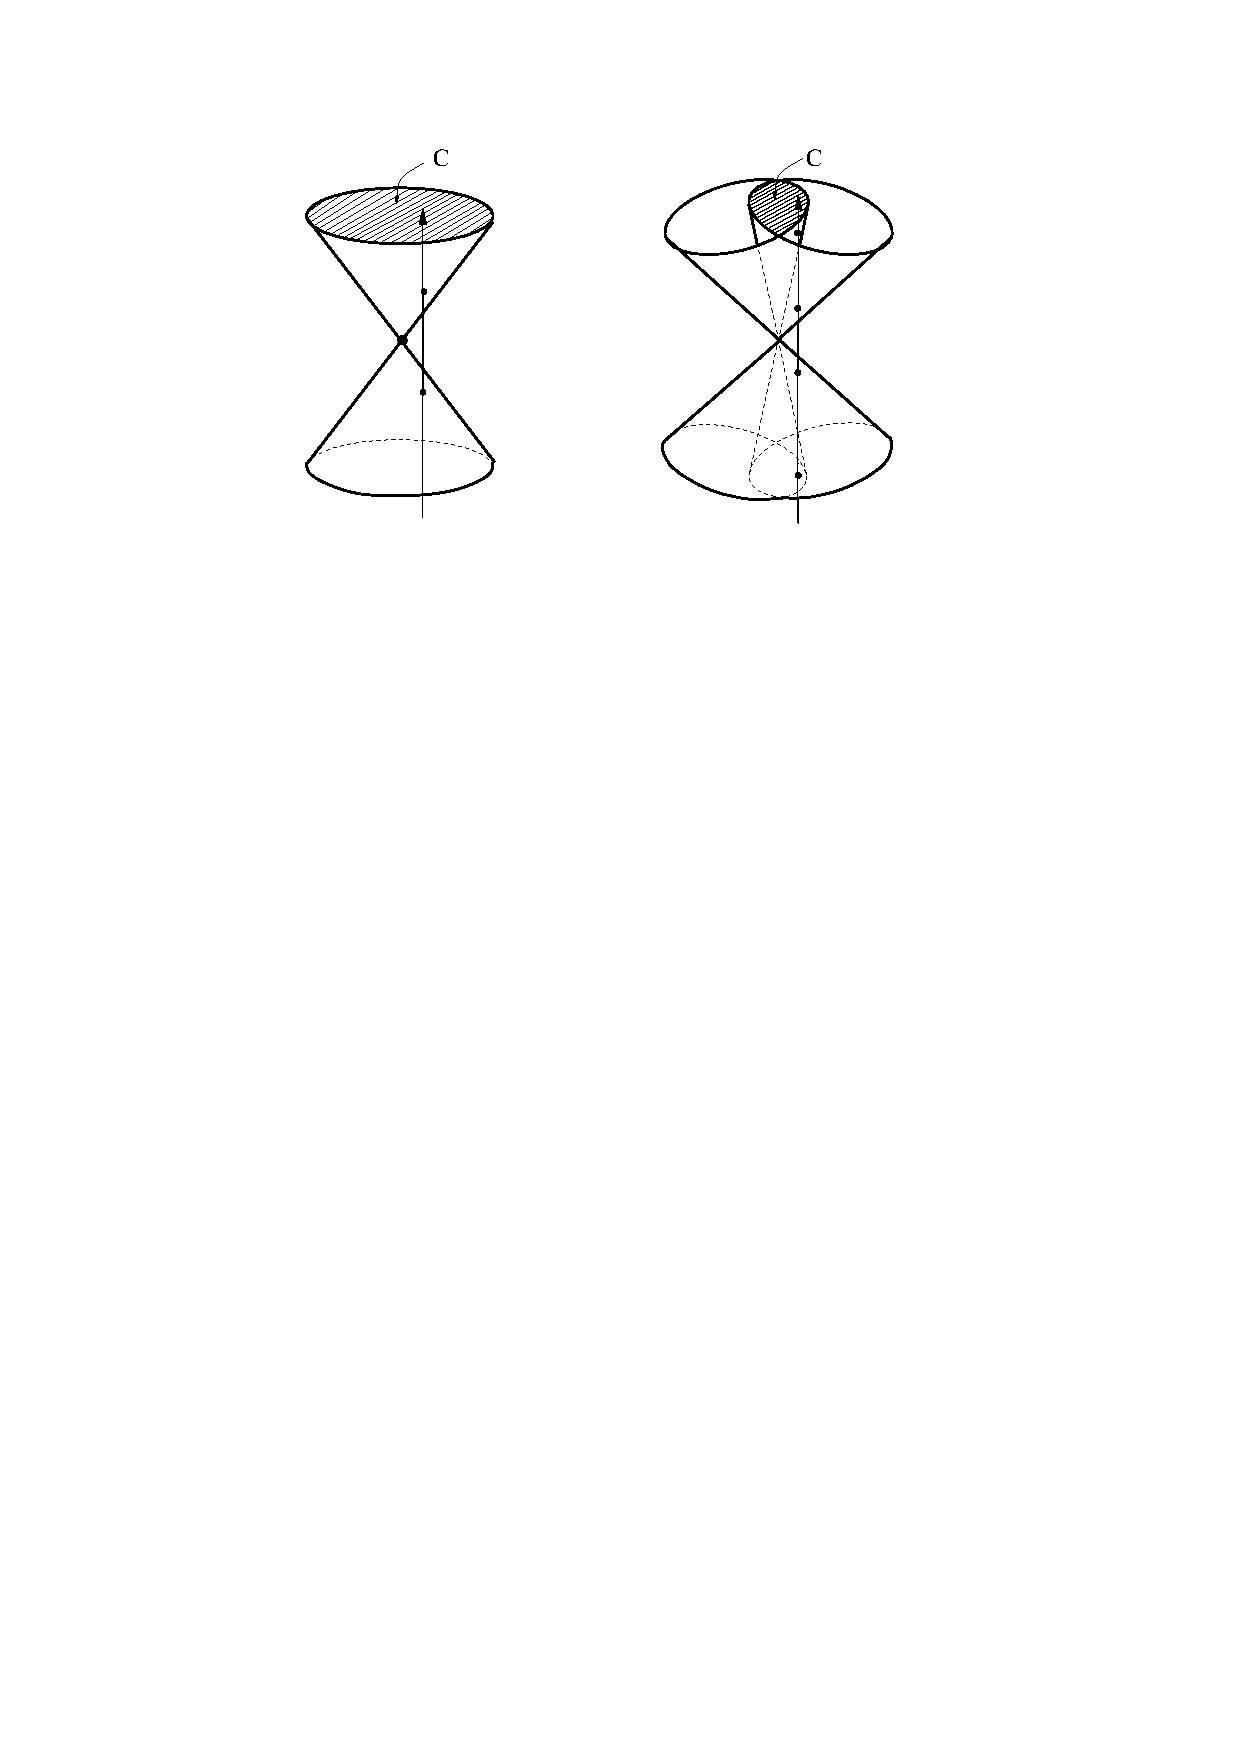
\includegraphics[width=\textwidth]{Poly.pdf}
    \caption{Hyperbolicity Cone and Vanishing Set of a Second and a Fourth Degree Polynomial (see \cite{Rivera}).}
    \label{hyperbol}
\end{figure}
One can now see the underlying geometric interpretation of  hyperbolic directions  $h\in \mathbb{R}^d$ for a given polynomial $P$. If $P$ is hyperbolic w.r.t. $h$ than any affine line in direction $h$ intersects $\mathrm{deg}(P) = d$ times with the vanishing set $V(P)$.

Finally, we can state the connection between hyperbolic polynomials and the well-posedness of the Cauchy problem.
\begin{theorem}
If the Cauchy-Problem of a given PDE is well-posed in a region of $M$, then the Principal Polynomial necessarily restricts to a hyperbolic polynomial on $T_p^{\ast}M$ for every $p$ contained in that region. Furthermore, exactly those hypersurfaces that have at every point a conormal which is hyperbolic w.r.t. $\mathcal{P}$ are admissible \textit{\textbf{initial data hypersurfaces}}, i.e., serve the purpose of specifying initial data.
\end{theorem}
\begin{proof}
The proof can be found in \cite{Hormander1977}\footnote{Much information is also contained in Hörmander's book series on partial differential equations (\cite{hormander1994analysis}, \cite{hormander2004analysis}, \cite{hormander2009analysis}, and \cite{hormander2015analysis}).} and also in \cite{Ivrii_1974}. 
\end{proof}
In the following, we proceed as before and select at each spacetime point a connected component of the set of hyperbolic covectors that is encoded by $\mathcal{P}$. We denote the thus provided hyperbolicity cone of the principal polynomial $\mathcal{P}$ at $p \in M$ as $C_p(\mathcal{P}) \subset T_p^{\ast}M$.
Moreover, we require that the choice of hyperbolicity cone varies smoothly w.r.t. the individual spacetime points, i.e., it is made in such a way that the following map:
\begin{align}
\begin{aligned}
\pi_{\mathcal{P}}: \{ C_p(\mathcal{P}) \ \vert \ p \in M\}=: C(\mathcal{P}) &\longrightarrow M\\
C_p(\mathcal{P}) &\longmapsto p,
\end{aligned}
\end{align}
defines a smooth subbundle $(C(\mathcal{P}), \pi_{\mathcal{P}}, M) \subset T^{\ast}M$.
Choosing such a hyperbolicity cone at each spacetime point distinguishes a specific, connected subset of possible initial data hypersurface conormals. These then can be used to define a smooth distribution of cones on the tangent bundle $C^{\#} \subset TM$. Details how is construction can be carried out are provided in \cite{Rivera} and also \cite{2012arXiv1211.1914K} for a slightly different approach.
The distribution of tangent space cones then encodes feasible future directions at the particular spacetime points.
Thus, in conclusion,  the choice of hyperbolicity cones endows the spacetime manifold $M$ with a \textit{\textbf{time orientation}} (cf. \cite{2012arXiv1211.1914K} and \cite{Rivera}).

In total, we can sum up the situation as follows: If we are given a predictive PDE ---in the sense that there exist hypersurfaces such that the corresponding Cauchy problem is well-posed--- then we can calculate the Principal Polynomial of this PDE. This Principal Polynomial is then necessarily hyperbolic. As shown above, the zero variety of the Principal Polynomial describes the propagation of waves in the infinite frequency limit. Furthermore, from the Principal Polynomial, we can compute the hyperbolicity cones. These then precisely encode the admissible initial data hypersurface of the given PDE.

The above consideration immediately opens up a problem that we are going to outline in the following. In the first section, we developed the necessary techniques that allowed us to phrase the requirement of diffeomorphism invariance in terms of a linear, first-order PDE. Given a particular spacetime geometry, i.e., given a field bundle $F_{grav}$, computing solutions to the corresponding equivariance equation (\ref{DiffeoEqn}) would yield a diffeomorphism invariant theory of gravity described by a Lagrangian for the gravitational field and the corresponding gravitational EOM.
If the theory of gravity is additionally required to be predictive, then the corresponding gravitational principal polynomial $\mathcal{P}_{grav}$ is hyperbolic.

On the other hand, in order to really put that theory to use and derive predictions meaningful predictions from it, that in particular can be probed in experiments, we additionally need a theoretical description of the matter that couples to that particular gravitational field and foremost also generates it.
This additional matter theory is then prescribed on top of the geometric background that is provided by the gravitational field. If we also require matter to be governed by predictive EOM than also the matter principal polynomial $\mathcal{P}_{mat}$ is necessarily hyperbolic.

More precisely, the situation now looks as follows:
As before, gravitational Lagrangian is given by a bundle map:
\begin{align}
    \mathcal{L}_{grav} : J^2F_{grav} \longrightarrow \Lambda^4M
\end{align}
Where $F_{grav}$ is the gravitational field bundle. Additionally we now also have a matter field described by a Lagrangian that depends on the values of the matter field and its first derivatives\footnote{We might also here consider the case where the Lagrangian also depends on second derivatives of the matter field and is thus required to be degenerate s.t. the matter EOM are again of second derivative order, but for simplicity, we restrict to first-order matter Lagrangians.}, but also exploits the spacetime geometry provided by the gravitational field. Thus the matter Lagrangian is a bundle map
\begin{align}
    \mathcal{L}_{mat} : F_{grav} \times J^1F_{mat} \longrightarrow \Lambda^4M,
\end{align}
where $F_{mat}$ is the matter field bundle. In the following we will denote adapted coordinates on $J^1F_{mat}$ by $(x^m,\phi^{\tilde{A}},\phi^{\tilde{A}}_m)$ Hence the total Lagrangian is given by:
\begin{align}
\begin{aligned}
    \mathcal{L}_{tot} : J^2F_{grav} \times J^1F_{mat} &\longrightarrow \Lambda^4M \\
    \mathcal{L}_{tot} &= \mathcal{L}_{grav} + \mathcal{L}_{mat}.
\end{aligned}
\end{align}
We now get two sets of EOM one from taking the variational derivative of $\mathcal{L}_{tot}$ w.r.t the gravitational field bundle coordinates, i.e., the gravitational EOM and one from taking the variational derivative w.r.t. the matter field bundle coordinates $\phi^{\tilde{A}}$, the matter EOM.
The gravitational EOM now feature an inhomogeneous term that describes how the matter sources the gravitational field.
\begin{align}
    0 = \frac{\delta \mathcal{L}_{tot}}{\delta v_A} = \frac{\delta \mathcal{L}_{grav}}{\delta v_A} + \frac{\delta \mathcal{L}_{mat}}{\delta v_A}.
\end{align}
The matter EOM is given by 
\begin{align}
    0 = \frac{\delta \mathcal{L}_{mat}}{\delta \phi^{\tilde{A}}}.
\end{align}
We can then compute the two Principal Polynomials that correspond to the two EOMs, $\mathcal{P}_{grav}$ and $\mathcal{P}_{mat}$. Note in particular that these will depend both on the values of the gravitational field. We denote the corresponding vanishing sets by $V_{p,grav}$ and $V_{p,mat}$. As we required both theories to be predictive, i.e., have well-posed Cauchy problems we can also compute the two hyperbolicity cones $C_{p,grav}$ and $C_{p,mat}$ that at each spacetime point $p\in M$ encode the possible choices of initial data hypersurfaces for the two theories. 

Doing this at given $p \in M$ we would now end up with one of the following three situations of which we will show in that only one can serve the purpose of describing a meaningful physical theory:
\begin{itemize}
    \item $C_{p,grav} \neq C_{p,mat}$ and $V_{p,grav} \neq V_{p,mat}$
    
This situation obviously incorporates the special case where the two hyperbolicity cones are disjoint. This case can be immediately ruled out as then there would not exist a single initial data hypersurface that is common to both theories and hence could serve as a starting point for solving the coupled matter gravity system.   

Also, if the two hyperbolicity cones are not disjoint but nevertheless do not coincide we immediately get problems. Then we would either find a suitable matter initial data hypersurface that is no admissible initial data hypersurface for the gravitational EOM, or vice versa we would find a gravitational initial data hypersurface that can not serve the purpose of specifying initial data for the matter EOM. As can be seen, for instance in \cite{Rivera}, and also in \cite{2011PhRvD..83d4047R} the hyperbolicity cones of a given EOM are in close relation with feasible observer definitions for the underlying theory. Any physically meaningful observer must be able to collect data in his spatial surroundings and use the EOM provided by the theory to evolve this initial data to future values and thereby make physical predictions. To allow for this process, the spatial surrounding of any possible observer must serve as initial data hypersurface. Hence if there exist initial data hypersurfaces that are exclusive to either the matter or the gravitational EOM, we would end up with certain observers that are limited to one of the two theories. Such observers could in particular meaningfully measure data and predict processes in the corresponding free theory, being either the matter theory or gravity, but become meaningless once the coupled case is concerned.

In the following we want to restrict to situations that allow for a unified observer definition, i.e., the observers of gravity and matter theory obey the same laws and in particular posses the same properties no matter if the two theories are coupled or one considers the case of a free treatment of either one independently. Hence we dismiss the case where $C_{p,grav} \neq C_{p,mat}$.

\item $C_{p,grav} = C_{p,mat}$ and $V_{p,grav} \neq V_{p,mat}$ 

In this case, all initial data hypersurfaces are common to both theories. Nevertheless, the vanishing sets of the two Principal Polynomials differ. We have seen that these vanishing sets govern the propagation behavior of wave-like solutions in the infinite frequency limit. It might hence be possible that, if $V_{p,grav} \neq V_{p,mat}$, the wave propagation of matter waves and gravitational waves shows quite different properties. The structure provided by the vanishing sets of the two Principal Polynomials, in particular, governs the information regarding future domains that such a propagating wave might causally influence — doing so it particular encodes the speed of such waves. 

With the recent detection of gravitational waves \cite{2017ApJ...848L..12A}, \cite{2017PhRvL.119n1101A} and \cite{2016PhRvL.116f1102A} also further insight regarding their propagating speed is gained rapidly. 
To provide an example using the observed time difference between the gravitational wave event GW170817 and the gamma-ray burst GRB 170817A emitted by a Binary Neutron Star Merger the propagation speed of gravitational waves has already be constrained to deviate no more than $-3\cdot 10^{{-}15}c$ and $+7\cdot 10^{{-}16}c$ from the speed of light $c$ (see \cite{2017ApJ...848L..13A}). Hence it seems reasonable to additionally require that $V_{p,grav} = V_{p,mat}$, in order to incorporate the thus already observed similarities in the propagation of gravitational and matter waves into our framework. We are therefore left with the final option.
\item $C_{p,grav} = C_{p,mat}$ and $V_{p,grav} = V_{p,mat}$ 

This situation is the only option left and henceforth precisely what we will require in the following. Not only all possible initial value hypersurfaces and therefore all possible observers of the matter and gravity EOM then coincide, but this option also requires that the causal structure in the form of wave propagation in the infinite frequency limit is the same for the two theories.  
\end{itemize}
\begin{remark}
Note that the requirement $V_{p,grav} = V_{p,mat}$ could be loosened to the point where we only impose that $V_{p,mat} \subset V_{p,grav}$. This would still be consistent with the measured propagation speed of gravitational waves, as then, in particular, every wave covector of the matter theory serves as wave covector of gravitational waves. Further wave covectors that are exclusive to gravitational waves do not necessarily contradict observations. Such waves might have simply not been detected, yet. This could, for instance, be explained if such covectors correspond to massive modes which thus decay faster and therefore are harder to observe in large distances from the source. Nevertheless restricting to $V_{p,grav} = V_{p,mat}$ for the future developments yet to come seems reasonable.
We will even see that at least in the two perturbative examples that we are going to treat in the next chapter, the two requirements are in fact equivalent.
\end{remark}
The previous investigation yields the second and last requirement that we wish to pose on the theory of gravity that we want to construct. We require that given a matter theory that employs the theory of gravity as geometric background, the two theories are \textit{\textbf{compatible}} in their \textit{\textbf{causal structure}} in the sense that the two Principal Polynomials at each point yield the same vanishing set, i.e., it holds for all $p \in M$ that: 
\begin{align}
    V_{p,grav} = V_{p,mat}.
\end{align}
Note that then $C_{p,grav} = C_{p,mat}$ immediately follows. Further note that the above condition, the equality of the two vanishing sets, simply requires the two polynomials to be compromised of the same irreducible polynomial factors. In most relevant cases, the factorization of the polynomials can easily be obtained.


Summing up the previous achievements, it is now conceptually apparent how we must proceed to find the most general gravitational Lagrangian that is compatible with any given matter theory. We first solve the equivariance equations (\ref{DiffeoEqn}) to implement the required diffeomorphism invariance of the theory of gravity paying close attention to make sure that the resulting EOM are of no higher than second derivative order. Then we compute the gravitational Principal Polynomial and compare it to the one obtained from the matter theory. We require that at each spacetime point the two polynomials define the same vanishing set and by this get further conditions the gravitational Lagrangian has to solve, this time encoding the causal compatibility between matter theory and gravity.
We end this section by formulating this results in terms of a definite construction manual that is displayed as the Algorithm \ref{Algo1}.
\begin{algorithm}[hbt!]
\SetAlgoLined
\KwData{Matter theory: $ \mathcal{L}_{mat} : F_{grav} \times J^1F_{mat} \longrightarrow \Lambda^4M$.
}
\KwResult{Most general diffeomorphism invariant, causal compatible theory of gravity: $\mathcal{L}_{grav} : J^2F_{grav} \longrightarrow \Lambda^4M$ .}
Compute the vertical coefficients $C^{Bm}_{An}$ of the infinitesimal diffeomorphism action on $F_{grav}$. \\
Set up the equivariance equations (\ref{DiffeoEqn}). \\
Solve the equivariance equations (\ref{DiffeoEqn}) to obtain the most general diffeomorphism invariant $L_{grav}(x^m,v_A,v_{Am},v_{AI})$.\\
Compute the EOM $\frac{\delta L_{grav}}{\delta v_A}$.\\
Consider the most general subtheory that has 2nd-order EOM.\\
Calculate the Principal Polynomials $\mathcal{P}_{grav}$ and $\mathcal{P}_{mat}$.\\
Determine the arbitrary quantities in $L_{grav}$ s.t. for all $p \in M$ : $V_{p,grav} = V_{p,mat}.$
 \caption{Construction of Gravitational Lagrangian}\label{Algo1}
\end{algorithm}


\section{Perturbative Approach to Constructive Gravity}
In the previous section, we have completed the required diffeomorphism invariance of the gravitational theory with the second requirement $V_{p,grav}=V_{p,mat}$ ensuring the compatibility with a given matter theory. Conceptually, it is therefore entirely clear how one can solve the problem posed by Constructive Gravity. Practically obtaining solutions to the diffeomorphism equivariance equations (\ref{DiffeoEqn}) is, however, a different question. Although the relevant PDE is linear in the unknown Lagrangian and furthermore only of first derivative order --- methods for solving  such PDEs have actually already been known for a long time (cf. \cite{Hilbert} and also \cite{Han2015}) --- already treating the standard case of finding the most general such Lagrangian that can be constructed from a metric tensor field and its first and second derivatives is surprisingly hard. The reason is the sheer size of the resulting PDE system. For the stated example of metric gravity we will later see that the PDE system is compromised of a total of 136 partial differential equations and the Lagrangian is a function of 150 independent variables.  

Regarding this, we are essentially left with one of two options that avoid the mammoth task of solving the equivariance equations in fully general form and nevertheless furnish us with access to two exceptionally relevant realms of gravitational physics. We can either apply \textbf{\textit{symmetry}} methods to the equivariance equations and thereby for a given gravitational field obtain solutions, i.e., theories of gravity that describe the relevant phenomenology under these symmetry assumptions. We could, for instance, solve the equivariance equation assuming spatial homogeneity and isotropy to obtain a description of cosmology in the generalized spacetime geometry.
Such an approach will be discussed in \cite{NilsPHD}.
Alternatively --- and this is the path that we will take in the following --- we can perturbatively solve the equivariance equations by employing the previously developed framework for computing \textit{\textbf{power series solution}} in some finite order. We, in particular, chose this path with the treatment of gravitational waves in mind.  The recent developments in the detection of gravitational waves makes them an excellent tool to test alternatives to GR \cite{2010PhRvD..81f4008Y}, \cite{2011PhRvD..83j4022B}, \cite{2017PhRvD..95j4027Z}, \cite{2013LRR....16....9Y}.

We have already gathered the necessary techniques that allow us to construct perturbative solutions to the equivariance equations in a rigorous fashion in the previous section. Primarily we have seen that such an approach only yields meaningful results if the relevant PDE is \textit{\textbf{involutive}}. We are now going to apply these techniques to the equivariance equations (\ref{DiffeoEqn}). To that end, it is vital to take a closer look at the jet bundle that underlies the geometric treatment of the PDE provided by (\ref{DiffeoEqn}). Recall that the Lagrangian in consideration is given by a bundle map:
\begin{align}
\mathcal{L} : J^2F \longrightarrow \Gamma^4M.
\end{align}
Abstractly the PDE (\ref{DiffeoEqn}) is then defined as a submanifold of the first-order jet bundle $J^1(J^2F \times \Lambda^4M)$ over the trivial bundle $J^2F \times \Lambda^4M$. 
We denote adapted coordinates on $J^1(J^2F \times \Lambda^4M)$ by $(x^m,v_A,v_{Am},v_{AI},l,l^{m},l^{A},l^{Am},l^{AI})$ such that we obtain the formal representation of the PDE (\ref{DiffeoEqn}) by replacing the bundle map $L$ the derivatives $L^{:m},L^{:A},...$ with fiber coordinates $l$ and derivative coordinates $l^m,l^A,...$. Hence in terms of formal PDE theory the equivariance equation reads 
\begin{align}\label{DiffeoEqnFormal}
\begin{aligned}
    0 &= l^{m} \\
    0 &= l^{A} C_{An}^{Bm} v_B + l^{Ap} \bigl[ C_{An}^{Bm} \delta_p^q - \delta_A^B \delta_m^n \bigr] v_{Bq} + l^{AI} \bigl[ C_{An}^{Bm} \delta_I^J - 2 \delta_A^B J_I^{pm} I^J_{pn}  \bigr] v_{BJ} + l \delta^m_n \\
    0 &= l^{A(p\vert}C_{An}^{B \vert m)} v_B + l^{ AI} \bigl[ C_{An}^{B(m\vert} 2 J_I^{\vert p) q} - \delta^B_A J_I ^{pm} \delta_n^q \bigr] v_{Bq} \\
    0 &= l^{AI} C_{An}^{B(m\vert} v_B J_I^{\vert p q )}.
    \end{aligned}
\end{align}

We begin the perturbative treatment of Constructive Gravity with one of the main results that in the end justifies the perturbative approach:
\begin{theorem}
PDE (\ref{DiffeoEqnFormal}) is involutive.
\end{theorem}
\begin{proof}
We start by proofing that the symbol of the equation (\ref{DiffeoEqnFormal}) is involutive. Since the PDE is of first derivative order its symbol simply consists of its homogeneous part, namely the PDE with the second equation being replaced by the homogeneous counterpart:
\begin{align}
    0 &= l^{A} C_{An}^{Bm} v_B + l^{Ap} \bigl[ C_{An}^{Bm} \delta_p^q - \delta_A^B \delta_m^n \bigr] v_{Bq} + l^{AI} \bigl[ C_{An}^{Bm} \delta_I^J - 2 \delta_A^B J_I^{pm} I^J_{pn}  \bigr] v_{BJ}.
\end{align}
This homogeneous system describes functions that are invariant under the action of any lifted vector field (\ref{LieJ2}). 

The first step in proving involution of the symbol is computing the sum of beta numbers. We have to pay attention as we have to compute this sum in coordinates that maximize it, i.e., are $\delta$-regular. However, because we are dealing with first-order equations, the classes of the derivative indices all posses exactly one member and range from 1 to $\mathcal{k}$ where 
\begin{align}
    \mathcal{k} := \mathrm{dim}(J^2F) = 4+n+4n+10n,
\end{align}
$n$ being as before the fiber dimension of $F$. 
In the following, we are going to assume that $\mathrm{dim}(J^2F)$ is bigger than the number of independent equations in (\ref{DiffeoEqnFormal}) which is given by 140 as otherwise, in general, there will not exist solutions in the first place. 
The maximum value for the sum of betas is obtained when we transform the coordinates on $J^2F$ s.t. the first equation is solved w.r.t. the derivative coordinate with maximal class $\mathcal{k}$ and the $i$th equation is solved w.r.t. the derivative coordinate of class $\mathcal{k}-i$ such that the last equation is solved w.r.t. the derivative coordinate of class $\mathcal{k}-139$.
Note that this immediately renders the symbol in solved form.
To simplify the notation in the following we briefly denote coordinates on $J^2F$ that bring the symbol to this form by $y_a$ for $a = 1,...,\mathcal{k}$, where the ordering is taken as $y_{\sigma} < y_{\tau}$ for $\sigma < \tau$. Moreover we denote the corresponding derivative coordinates by $l_{\sigma}$. 
Note that such coordinates always exist. 
If we display the symbol $M_1$ as matrix and sort its columns by class starting from the highest class $\mathcal{k}$ and further label its rows by the individual equations, from 1 to 140, this transformation this coordinate transformation on $J^2F$ corresponds to bringing the matrix to the following upper triangular form
\begin{align}\label{symbolMat}
\begin{blockarray}{cccccccccc}
\underset{\longrightarrow}{\text{class}} & \mathcal{k} & \mathcal{k} -1 & \hdots & \hdots & \hdots & \mathcal{k}- 140 & \hdots & 1 & \downarrow \text{Equation} \\
\begin{block}{c(cccccccc)c}
   & 1 & a^1_{\mathcal{k}-1} & \hdots & \hdots & \hdots & a^1_{\mathcal{k} -140} & \hdots & a^1_1 & 1 \\
    & 0 & \ddots & \ddots & &  & \vdots & & \vdots & \vdots \\
    & \vdots & \ddots  & \ddots & \ddots &  & \vdots & & \vdots & \vdots \\
    & \vdots & & \ddots & \ddots & \ddots & \vdots & & \vdots &  \vdots\\
    & 0 & \hdots  & \hdots & 0 & 1 & a^{140}_{\mathcal{k}-140} & \hdots & a^{140}_{1} &  140 \\
\end{block}
\underset{\longrightarrow}{\text{coordinate}} & l_{\mathcal{k}} & l_{\mathcal{k} -1} & \hdots & \hdots & \hdots & l_{\mathcal{k}- 140} & \hdots & l_1 &
\end{blockarray}
\end{align}
for some $a^{\alpha}_{\tau}$ that are functions on $J^2F$ . The sum of betas can then be computed to be given by:
\begin{align}
    \sum_{i=1}^{\mathcal{k}} i \beta_1(i) = \sum_{i = 0}^{139} \mathcal{k} - i .
\end{align}
We now have to show that this equals the rank of the prolonged symbol $M_2$. By previous arguments, this is the case if we obtain all equations of $2$nd derivative order by prolongations w.r.t. multiplicative variables only. We again consider the symbol solved to the form given by matrix (\ref{symbolMat}). 
We take an arbitrary row $\sigma$, for $\sigma=1,...,140$, and consider the corresponding equation $E_{\sigma}$. The multiplicative variables of this $\sigma$th equation are $y_1,...,y_{\mathrm{cls}(\sigma)}$ where we introduced 
\begin{align}
\mathrm{cls}(\sigma):= \mathcal{k} - \sigma +1.
\end{align}
In other words $\mathrm{cls}$ returns the class of a given row
We now show that prolonging this equation w.r.t. an arbitrary non multiplicative variable $y_b$ for $b>\mathrm{cls}(\sigma)$ yields no additional independent contribution to the prolonged symbol. This is achieved by showing that we can add prolongations w.r.t. multiplicative variables to such a non multiplicative prolongation $D_bE_{\sigma}$ and thereby obtain an equation of first derivative order which is thus not present in $M_2$. Note that in the matrix (\ref{symbolMat}) multiplicative variables of a given row are exactly those corresponding to the columns that are right to the normalized pivot elements (including these) and thus contain the functions $a^{\alpha}_{\tau}$. Non-multiplicative variable correspond to the columns left to the pivots that hence contain only zeros.

Prolonging $E_{\sigma}$ w.r.t. such a $y_b$, i.e., computing $D_bE_{\sigma}$ we get second-order derivatives of the form $y_{bc}$ for $c < \mathrm{cls}(\sigma)$, where $y_c$ is multiplicative for $E_{\sigma}$. Considering a particular such $c$ as an example, we can now get rid of this second order derivative contribution by utilizing the equation with pivot of class $b$. As $b>c$ such an equation necessarily exists; this can easily be seen from the upper triangular structure of the solved symbol. More precisely this equation is explicitly given by $E_{\mathrm{cls}(b)}$.
Since $c<b$, $y_c$ is multiplicative for $E_{\mathrm{cls}(b)}$. We prolong $E_{\mathrm{cls}(b)}$ w.r.t. $y_c$, scale it appropriately, by the negative of the coefficient of $l_{bc}$ in the previously computed non multiplicative prolongation $D_bE_{\sigma}$ and add it to this equation. Doing so we remove the entire contribution from $y_{bc}$. Similarly, one can get rid of all further second derivative contributions contained in $D_bE_{\sigma}$. In total we therefore see that we can add multiplicative prolongations to remove the whole second derivative order of such a non multiplicative prolongation $D_bE_{\sigma}$.
Hence any non multiplicative prolongation does not contribute an independent new second-derivative-order equation to the prolonged symbol $M_2$ and the symbol. The symbol is therefore involutive. 

To proof that not only the symbol but also the PDE (\ref{DiffeoEqnFormal}) itself involutive, we have to show that the PDE generates no integrability conditions after one prolongation. We have already discussed that prolonging each equation only w.r.t. its multiplicative variables never produces integrability conditions. Furthermore, we have just shown that any prolongation w.r.t. non-multiplicative variables can be reduced to first derivative order by adding further multiplicative prolongations in the way it is outlined above. Hence the question is if the first derivative order contributions that we get from such a procedure are already included in $R_1$ or contribute additional independent equations. 

We first consider the homogeneous case. We take again the $m$th equation and work as before in the coordinates $y^a$ on $J^2F$ that solve the symbol $M_1$ to (\ref{symbolMat}). Note that this homogeneous linear first-order PDE can then be concisely written as
\begin{align}
    E_{\sigma} = l_{\mathrm{cls}(\sigma)} + \sum_{i = \sigma}^{\mathcal{k}} a^{\sigma}_{\mathrm{cls}(i)} l_{\mathrm{cls}(i) } .
\end{align}
We can equivalently write this in the form of vector fields on $J^2F$. We define for $\sigma = 1,...,140$ the vector fields $\zeta_{\sigma} \in \Gamma(J^2F) $ corresponding to $E_{\sigma}$:
\begin{align}
    \zeta_{\sigma} := \frac{\partial}{\partial y_{\mathrm{cls}(\sigma})} + \sum_{i = \sigma}^{\mathcal{k}} a^{\sigma}_{\mathrm{cls}(i)} \frac{\partial}{\partial y_{\mathrm{cls}(i)}}.
\end{align}
The solutions to the given homogeneous PDE are then precisely those functions on $J^2F$ that are invariant under these vector fields, i.e., that satisfy $\zeta_{\sigma} f = 0$ for all values of $\sigma$.
Note that we obtained the homogeneous PDE from precisely such an invariance requirement. The only difference to the previous case is that we now work coordinates that render the symbol particularly simple. 
In terms of vector fields this corresponds to the fact that the $\zeta_{\sigma}$ commute (see also \cite{seiler1994analysis}):
\begin{align}
    \left [ \zeta_{\sigma}, \zeta_{\tau}\right ] =0.
\end{align}

Carefully analyzing the above procedure, we now find that the remaining first-order equation that is produced when eliminating all second-order contributions of a non-multiplicative prolongation $D_bE_{\sigma}$ by multiplicative prolongations is simply given by the commutator equation
\begin{align}
    \left [\zeta_{\sigma}, \zeta_{\mathrm{cls}(b)} \right] = 0.
\end{align}
Hence for the system to not produce integrability conditions this commutator must now be given by a linear combination of unprolonged equations. For the particular case of the $\zeta_{\sigma}$, this is trivially true as the commutator of two such fields vanishes. This can, however, already be seen from the original system (\ref{DiffeoEqnFormal}).
Recalling that we obtained homogeneous counterpart to (\ref{DiffeoEqnFormal}) by requiring invariance under the prolonged vector fields $\xi_{J^2F}$ (\ref{LieJ2}) that were in particular constructed via a Lie algebra morphism. It is therefore clear that also these vector fields close under the operation of taking commutators. Hence no integrability conditions are generated, and the homogeneous system is involutive.

This is no special property of the homogeneous PDE in consideration but is actually general to all linear homogeneous first-order PDEs. Such PDEs that can be described entirely by vector fields are called \textit{\textbf{complete}} if the vector fields that generate the given system form a Lie algebra w.r.t. the commutator. If the vector fields commute, the system is furthermore called a \textit{\textbf{Jacobian}} system. One can show along the same lines that we followed her that in fact, any complete system is involutive. For details regarding the treatment of complete systems and in particular for a proof of this last statement see \cite{seiler1994analysis} and also for further information \cite{Clebsch1866}, \cite{caratheodory1956variationsrechnung} and \cite{lie1970theorie}.

What remains to show is that the presence of the inhomogeneity in $(\ref{DiffeoEqnFormal})$ does not change this observation, i.e., does not generate integrability conditions. We again work in the coordinates $y_a$. The inhomogeneity is only present in the equations $5-20$ and only when the indices in (\ref{DiffeoEqnFormal}) are such that $m = n$. We label the equations s.t. it contributes to equation $5,9,13$ and $17$. In each case, the contribution is simply given by an extra term of $+l$ and the respective equations $\Tilde{E}_{\sigma}$ of the inhomogeneous PDE read now 
\begin{align}
     \tilde{E}_{\sigma} = \begin{cases}
     E_{\sigma} + l \ &\text{for} \ \sigma \in \{ 5,9,13,17 \}\\
     E_{\sigma} \ &\text{else}.
     \end{cases}
\end{align}
One can now show along the same lines we followed in the homogeneous case that the inhomogeneous system is involutive if for any two such equations $\tilde{E}_{\sigma}$ and $\tilde{E}_{\tau}$ the so-called \textit{\textbf{Jacobi brackets}} or sometimes also called Mayer bracket 
\begin{align}
  \llbracket \tilde{E}_{\sigma}, \tilde{E}_{\tau} \rrbracket = \sum _{i = 1}^{\mathcal{k}} \biggl(\frac{\partial \tilde{E}_{\sigma}}{\partial l_i}\biggr) D_{i}\tilde{E}_{\tau} -  \biggl(\frac{\partial \tilde{E}_{\tau}}{\partial l_i}\biggr) D_{i}\tilde{E}_{\sigma} 
\end{align}
vanish on $R_1$ (see  \cite{seiler1994analysis} and also also Example 2.3.12 in \cite{seiler2009involution}), i.e., can be obtained by linear combinations of unprolonged equations. Comparing this to the previous case where the possible integrability conditions where built from the commutator we now get extra terms whenever either $\sigma$, $\tau$ or both are contained in $\{ 5,9,13,17 \}$. Consider first the case where $\sigma \in \{5,9,13,17\}$ but not $\tau$, then we have $\tilde{E}_{\sigma} = E_{\sigma} + l$ and $\tilde{E}_{\tau} = E_{\tau}$ and hence using the linearity of the Jacobi bracket
\begin{align}
    \llbracket \tilde{E}_{\sigma}, \tilde{E}_{\tau} \rrbracket = \llbracket E_{\sigma}, E_{\tau} \rrbracket - \sum_{i=1}^{\mathcal{k}} \frac{\partial E_{\tau}}{\partial l_i} l_i.
\end{align}
We can now use that the first contribution vanishes, $\llbracket E_{\sigma}, E_{\tau} \rrbracket = 0$ as this again essentially nothing different but the commutator of the two vector fields $[\zeta_{\sigma},\zeta_{\tau}]$ expressed in terms of the quantities $E_{\tau}$ and $E_{\sigma}$. We are thus left with the second term $- \sum_{i=1}^{\mathcal{k}} \frac{\partial E_{\tau}}{\partial l_i} l_i$, but as the equation $E_{\tau}$ is in particular linear in the $l_i$ this again yields $E_{\tau}$ and hence vanishes on $R_1$. Along the same lines one can proceed with the case of $E_{\tau}$ also containing extra contributions from $+l$. In total we thus find that also the inhomogeneous PDE is involutive which proofs the statement.
\end{proof}

We can now apply the previously developed techniques to obtain a power series solution to the PDE (\ref{DiffeoEqnFormal}). This then yields a finite order power series expansion of the requested gravitational Lagrangian of which we can, of course, compute the Euler Lagrange equations in the appropriate perturbative order. In other words, we thus get a perturbative theory of gravity. We consider the result that the PDE (\ref{DiffeoEqnFormal}) is involutive to be essential for this approach as only now as we have proven that we can be sure the contribution to the perturbative Lagrangian that we compute up to some finite order will not change in any higher-order of the power series procedure. Differently stated only with the PDE being involutive we can be sure to really extract all the for the particular order relevant information from it and not end up with a solution that is too general. 

Note that from the point of view of formal theory, involution of a PDE is not only essential for the construction of power series solution. Previously we have already stated that one of the key ideas behind a PDE with involutive symbol lies in the fact that one is then able to predict the rank of the prolonged symbol by means of (\ref{sumBeta}) without actually having to compute the relevant prolongations. As for an involutive symbol according to (\ref{invoCons}) also all prolonged symbols are involutive one can thus obtain formulae that also allow for the prediction of the ranks of higher-order prolongations of the symbol. Recall that the rank of the symbol $M_q$ essentially determines the number of expansion constants of order $q$ the one might specify arbitrarily when constructing a power series solution to the PDE  and thereby the various ranks of the symbol govern the entire information regarding the solution space of the given PDE.
Thus the involution of the PDE (\ref{DiffeoEqnFormal}) allows us to formulate the following statement about its general solution for arbitrary field bundles $F$.
\begin{theorem}\label{GeneralSol}
Given any field bundle $F$ with fiber dimension $n$. The general solution to the invariance equation, i.e., the homogeneous version of (\ref{DiffeoEqnFormal}) admits the form:
\begin{align}
    \mathcal{F} \left (\Psi_1,...,\Psi_r \right ),
\end{align}
where $r:=\mathcal{k}-140$, $\Psi_1,...\Psi_r$ are $r$ functionally independent solutions of the homogeneous PDE and $\mathcal{F}$ is an arbitrary function of these independent solutions. The general solution to the equivariance equation, i.e., the inhomogeneous PDE (\ref{DiffeoEqnFormal}) is given by:
\begin{align}
    \omega \cdot \mathcal{F} \left (\Psi_1,...,\Psi_r \right ),
\end{align}
where $\omega$ is any explicit solution of the PDE. 
\end{theorem}
\begin{proof}
The proof of the first statement is given by Proposition 7.1 in \cite{seiler1994analysis}. Further information can in particular be found in chapter 3 of \cite{seiler2009involution} and \cite{articleCH}. 

The second statement then simply follows from the previously stated fact that given an arbitrary solution $\mathcal{F}$ of the homogeneous PDE, multiplying by any solution $\omega$ of the inhomogeneous system yields again a solution of the inhomogeneous system and vice versa the quotient of any two solutions of the inhomogeneous PDE defines again a solution of the homogeneous system. The first part of this statement is simply a result of the linearity of the given PDE. For simplicity, we consider the case of a single equation 
\begin{align}
    0=D_i l + l 
\end{align}
and the corresponding homogeneous version. The generalization to finitely many equations is then really straight forward. 
We assume that we have the general solution of the homogeneous equation, i.e., $0 = D_i \mathcal{F}$ and also an explicit solution to the inhomogeneous version: $0 = D_i \omega + \omega$.
We first show that $\omega \cdot \mathcal{F}$ then also solves the inhomogeneous system. Inserting $\omega \cdot \mathcal{F}$ into the inhomogeneous PDE we get  
\begin{align}
    0 = \left ( D_i \mathcal{F} \right ) \cdot \omega + \mathcal{F} \cdot \left ( D_i \omega \right) + \mathcal{F} \cdot \omega. 
\end{align}
As $\mathcal{F}$ is supposed to provide a solution of the homogeneous equation, the first term vanishes. As $\omega$ solves the inhomogeneous equation the second term yields $\mathcal{F} \cdot \left ( - \omega \right )$,
and thus cancels the third term. We thus have shown that $\omega \cdot \mathcal{F}$ solves the inhomogeneous system. To complete the proof we still have to show that any solution of the inhomogeneous PDE is necessary of this form. We proof this by first taking an arbitrary solution of the inhomogeneous system $\rho$. We now take any other solution $\omega$ and insert the quotient $\rho/\omega$ into the homogeneous PDE
\begin{align}
    0 = D_i \left (\frac{\rho}{\omega} \right) = - (\frac{\rho}{\omega}) - \frac{\rho}{\omega^2} \cdot (-\omega) ,
\end{align}
Where we used $D_i \rho = -\rho$ and the same for $\omega$ as they both are supposed to solve the inhomogeneous system. Hence the quotient solves the homogeneous system. Obviously, we can write the solution $\rho$ as 
\begin{align}
    \rho = \omega \cdot  \frac{\rho}{\omega}.
\end{align}
However, as the first factor is taken to be a solution of the inhomogeneous system and we have now shown that the second factor solves the homogeneous PDE this is precisely the form that was claimed. 
Hence in total, we have thus shown that any solution of the inhomogeneous PDE is of the form $\omega \cdot \mathcal{F}$.
The straight forward generalization of this to the case finitely many PDEs then completes the proof.
\end{proof}
It is essential to observe that the previous theorem not only tells us the general form any solution to the equivariance or invariance equations respectively will admit but also provides us with information regarding the number of functionally independent solutions to these systems. Concretely for any field bundle, there will be 
\begin{align}
    \mathrm{dim}(J^2F) - 140 
\end{align}
functionally independent solution.
Therefore we see that the size of the space of potential candidates for a particular diffeomorphism invariant theory of gravity described in terms of a specific field bundle essentially depends only on the fibre dimension of the field bundle. 
This is obviously something that one might intuitively guess as it is merely the difference between the number of independent variables in $J^2F$ and the number of equations in the PDE. However only now that we know the equations are involutive we can be sure that there is no further information hidden in them yielding possibly additional restrictions on the unknowns and thereby reducing the number of functionally independent solutions. 
The proof of the involution of the equivariance equations is in particular not a mere technicality, but involution of this PDE could have made the difference between finitely many functionally independent solutions and not a single solution at all. 

Note that these solutions now, in general, will correspond to Lagrangians that might generate $4$th-derivative-order EOM. 
In the context of GR, these functionally independent solutions of the homogeneous equations are called \textit{\textbf{curvature invariants}}. In most cases, they are constructed from the Riemann curvature tensor. Observe, however, that also her the Riemann curvature is strictly speaking not necessary to obey such a notion of curvature invariants. 
In GR it is a well-known result that there exist 14 functionally independent curvature invariant, yet already for this rather simple case their concrete expressions are surprisingly difficult. Obtaining possible generating sets that allow one to express arbitrary other invariants in terms of them is still a topic of research. 
Moreover, note that computing a set of $14$ functionally independent curvature invariants is completely equivalent to solving the equivariance equation for the case of the metric field bundle.
In the context of GR the curvature invariants and also possibly higher invariants involving higher derivatives of the metric tensor are then mostly used to classify spacetimes. Details can be found in
\cite{2009CQGra..26b5013C}, \cite{Zakhary1997}, \cite{2002IJMPD..11..827C} and also \cite{doi:10.1063/1.531425}.

With our developed framework we can easily reproduce the known result of $14$ curvature invariants for GR. The fiber dimension of the bundle of symmetric $(0,2)$ tensors $F_{GR}$ is obviously 10 yielding for this case 
\begin{align}
    \mathrm{dim}(J^2F_{GR}) = 4 + 10 + 40 + 100 = 154,
\end{align}
which according to the above considerations, yields $154-140=14$ functionally invariant solutions.
Furthermore, we are now in a position where we can easily determine the number of curvature invariants for any other spacetime geometry, i.e., any other possible gravitational field. In order to do so we, in particular, do not need to rely on structural analogues to the Riemann curvature tensor.
When constructing particular alternative gravity theories,
such a prediction regarding the number of possible curvature invariants that a given spacetime geometry might admit yields vital information about the richness of the spacetime structure. 
Doing so we can obtain a first hint on how many undetermined quantities such a theory might feature, be it undetermined functions in a full formulation or undetermined parameters in a perturbative treatment.
Also we can then immediately compare the strength of any further condition that is posed on the theory of gravity --- in the sense of how many otherwise unknown quantities the condition  determines ---
to the fundamental requirement of diffeomorphism invariance.
We will further treat these ideas in a particular example that we will consider in the next chapter.

Before we concretely work out a general framework for computing perturbative solutions to the equivariance equations we concern ourselves for a moment with the question of what points $p_0 \in J^2F$ might serve as expansion points for such a power series. From the sheer mathematical point of view, there is really no restriction on the possible expansion points. Yet from a physical point of view, the specific expansion point will, in the end, determine the interpretation and foremost the range of validity of the thereby constructed perturbative theory of gravity. 

As we want to work towards the treatment of gravitational waves, we are going to restrict ourselves to certain expansion points that describe a \textit{\textbf{flat}} variant of the theory of gravity at hand. Solutions of the obtained perturbative equations can then be thought of as corrections to that flat background theory with the special case of gravitational waves being wave-like solutions that propagate on the given background. More precisely with a slight adaption of the usual meaning in Riemannian geometry\footnote{In Riemannian geometry one call a Riemannian manifold flat if the associated Riemannian curvature tensor vanishes everywhere. The existence of coordinates in which the derivatives of the metric are zero is then a consequence (see \cite{petersen2006riemannian}).} we call a section $G \in \Gamma(J^2F)$ \textit{\textbf{flat}} if there exist adapted coordinates on $J^2F$ s.t. the coordinate expression of $G$ satisfies $\partial_mG_{A}=0$.
Hence we chose an expansion point with adapted coordinates $(x_0^m,N_A,0,0)$. note that such a point is essentially already determined by a point in $F$. 

We are in particular interested in the case where the expansion point is not only flat but furthermore supports our intuition that the geometry of spacetime is in quite good approximation provided by the flat Minkowski metric $\eta_{ab} = \mathrm{diag}(-1,+1,+1,+1)$. 
%check signature !!!
%
%
In other words, we want to interpret solutions of the to-be-constructed perturbative theory of gravity as corrections to a flat Minkowski background. Note we are not restricting our treatment to metric theories of gravity but deliberately want to allow for more general tensor fields as spacetime geometry.
The interpretation of doing perturbation theory around Minkowski spacetime will nevertheless become meaningful once the additional matter theory $\mathcal{L}_{mat}(x^m,\phi^{\tilde{B}},\phi^{\tilde{B}}_m,G_A)$ is provided. We then require from our flat expansion point that the specific matter theory defined on this flat expansion background $\mathcal{L}_{mat}(x^m,\phi^{\tilde{B}},\phi^{\tilde{B}}_m,N_A)$ is equivalent to the counterpart that we get when placing the matter field $\phi^{\tilde{B}}$ on a Minkowski background. 
In most cases this is achieved by constructing $N_A = N_A(\eta_{ab})$ from the Minkowski metric. We call such expansion points in the following \textit{\textbf{$\boldsymbol{\eta}$-induced}}.

Note that this clearly restricts the set of field bundles $F$ we can possibly treat to those that are compromised of tensors with an even total rank, as we simply cannot write down expressions with odd rank that are solely constructed from $\eta_{ab}$. This will not affect any further developments as in all examples we will treat, the gravitational field is described by an even rank tensor field. There are even certain arguments mainly stemming from QFT that the gravitational field must be of even rank in order to describe an attractive force (see for instance \cite{vecchiato2017variational}). 

We start our development of a framework that will allow us to construct perturbative expansions of diffeomorphism invariant Lagrangians for arbitrary fields by writing down the general finite power series expansion of an arbitrary such Lagrangian up to some order $r > 0$ around a flat expansion point $p_0 \in J^2F$ with adapted coordinates $p_0 \equiv (x_0^m,N_A, 0, 0)$. Note again that such a Lagrangian is already a bundle map on the second-order jet bundle $J^2F$, the equivariance PDE (\ref{DiffeoEqnFormal}) is then constructed as a submanifold of $J^1(J^2F \times \Lambda^4M)$. It is important not to confuse the two different ways the jet bundle construction is involved therein. In order to concisely display such a power series Lagrangian, we need to agree on some further notation. We denote the adapted coordinates on $J^2F$ collectively by
\begin{align}
    (v_{AI_k}) := (x^m,v_A,v_{Ap},v_{AI}).
\end{align}
In order to distinguish the appearing derivative indices $I_k,J_k,...$ that label higher spacetime derivatives from those that label higher derivatives w.r.t. the fiber coordinates of $J^2F$ we denote the latter ones by letters
$\tilde{I}_k, \tilde{J}_k$, ... . Finally we introduce the coordinate expression of the deviation from the expansion point 
\begin{align}
    (H_{AI_k}) := (v_{AI_k}) - (N_{AI_k}) = (x^m-x_0^m,v_A-N_A,v_{Ap},v_{AI}).
\end{align}

Before we write down the concrete expression for the expansion of the Lagrangian note that the first equation in (\ref{DiffeoEqnFormal}) simply states that the Lagrangian must not explicitly depend on $x^m$, hence we can discard any explicit $x^m$ dependency from the very beginning and therefore also exclude such from the power series expansion. In total, with the introduced notation, a general power series expansion reads as follows. 
\begin{align} \label{generalPowerSL}
    \begin{aligned}
    &L_{per}  \mathrm{d}^4x = \mathcal{L}_{per} : J^2F \longrightarrow \Lambda^4M \\
    &L_{per} = \sum_{n=0}^r \sum_{k_1,...,k_n = 0}^2 a^{\tilde{I}_k} \cdot J_{\tilde{I}_k}^{A_1I_{k_1}...A_nI_{k_n}} H_{A_1I_{k_1}} \cdot ... \cdot H_{A_nI_{k_n}}
    \end{aligned}
\end{align}
%rewrite this ???
%
%
As before the $a^{\tilde{I}_k}$ are constants.
We further define a second way of displaying these constants:
\begin{align}
    a^{A_1I_{k_1}...A_nI_{k_n}} := a^{\tilde{I}_k} \cdot J_{\tilde{I}_k}^{A_1I_{k_1}...A_nI_{k_n}}
\end{align}
In order to clarify this last expression further, we now explicitly provide the first three orders of this expansion. For that particular case, we drop any numerical factors due to the intertwiners as this simply corresponds to redefining the constants. Furthermore, we split the sums over the $v_{AI_{k_i}}$ into the different contributions of $(v_A,v_{Ap},v_{AI})$:
\begin{align}\label{LPert}
\begin{aligned}
    L_{per} = \  &a_0 + a^A H_A + a^{Ap} H_{Ap} + a^{AI}H_{AI} + a^{AB} H_{A}H_{B} + a^{ABp}H_A H_{Bp} + a^{ABI} H_{A} H_{BI}\\
    &+a^{ApBI}H_{Ap} H_{BI} + a^{AIBJ} H_{AI}H_{BJ} + a^{ABC} H_a H_B H_C 
    + a^{ABCp} H_A H_B H_{Cp} \\
    &+a^{ABCI} H_A H_B H_{CI} + a^{ABpCq} H_{A}H_{BP}H_{Cq} + a^{ABpCI} H_A H_{Bp} H_{CI}\\
    &+ a^{ABICJ} H_A H_{BI}H_{CJ} 
    + a^{ApBqCm} H_{Ap} H_{Bp} H_{Cm}+ a^{ApBq CI} H_{Ap} H_{BP} H_{CI}\\
    &+ a^{Ap BI CJ} H_{Ap} H_{BI} H_{CJ} + a^{AIBJCK} H_{AI} H_{BJ} H_{CK} + \mathcal{O}(4),
\end{aligned}
\end{align}
where $\mathcal{O}(4)$ denotes terms that are of order four or higher in any $(H_{AI_k})$. We now proceed exactly as outlined before in calculating the perturbative solution to solution to (\ref{DiffeoEqn}) from the above power series ansatz of the Lagrangian. We start by plugging in the expansion (\ref{LPert}) into the PDE (\ref{DiffeoEqnFormal}) and evaluate at the expansion point $p_0$. Note that evaluating at $p_0$ in coordinates corresponds to evaluating at $(H_{AI_k})=0$. This then yields equations for the expansion constants $a_0, a^A, a^{Ap}$ and $a^{AI}$. To obtain equations for the remaining higher-order expansion coefficients, we simply prolong the PDE and again insert the series expansion and evaluate at $p_0$. As we have shown that PDE (\ref{DiffeoEqnFormal}) is involutive, there will not occur any integrability conditions.

There is, however, one obstruction to this procedure that will become noticeable by providing additional lower-order equations that are revealed only after prolongations, yet they have nothing to do with integrability conditions. 
The reason for this obstruction is that the chosen $\eta$-induced expansion point in general features higher symmetry than an arbitrary point in $J^2F$. More precisely since we required $N_A(\eta_{ab})$ to be constructed from the Minkowski metric through products, sums and possibly contractions, it is \textit{\textbf{Lorentz invariant}}. To further investigate the consequences thereof we consider first an arbitrary flat expansion point $\tilde{p}_0 \in J^2F$ with coordinates $(\tilde{x}_0^m,M_A,0,0)$. Evaluating the second equation in (\ref{DiffeoEqnFormal}) for this point yields:
\begin{align}
    0 = l^A \vert _{\tilde{p}_0} C^{BM}_{An}M_B.
\end{align}
When evaluated at a general point, these are 16 independent equations. 
Conversely evaluating the same equation at the $\eta$-induced expansion point we find that:
\begin{align}\label{RankDef}
    0 = l^A \vert_{p_0} C^{BM}_{An}N_B
\end{align}
provides only 10 independent equations. The reason for this rank defect and foremost, its connection to the observed Lorentz invariance can be observed by considering the expression $K_{m[rs]}^n :=\eta_{m[r}\delta_{s]}^n$. 
Taking a closer look at the six individual expressions that can be obtained from the six possible values of the anti symmetric index pair  $\{K_{m[rs]}^n \ \vert \ r < s \} $ we find that they all are by construction anti symmetric w.r.t. the Minkowski metric, i.e., they satisfy 
\begin{align}
K_{m[rs]}^n\eta_{n p} - m \leftrightarrow p = 0.
\end{align}
Furthermore, they are all linearly independent when identified as real $4 \times 4$ matrices. Considering the dimension of the vector space of $4 \times 4$ matrices that are anti symmetric w.r.t. the matrix expression of $\eta_{ab}$ we find that  the expressions $K_{m[rs]}^n$ even constitute a basis of the vector space of $\eta$-antisymmetric matrices. 

One can show that the Lie algebra of the Lorentz group $SO(1,3)$ is isomorphic to the Lie algebra that is obtained by equipping this vector space of $\eta$-antisymmetric matrices with the standard matrix commutator. Hence these six matrices actually yield a basis of the Lie algebra $\mathrm{Lie}(SO(1,3))$. One often calls such matrices the \textit{\textbf{generators}} of the corresponding group as finite group elements can be obtained by applying the exponential map to linear combinations of them. Much information regarding the Lorentz group can be found in \cite{doi:10.1142/p199} and \cite{naimark2014linear}.

It is now clear that it henceforth holds that
\begin{align}
    0 = C^{Bm}_{An}N_B K_{m[rs]}^n,
\end{align}
as this is nothing but the infinitesimal change of $N_A$ under Lorentz transformations, but as $N_A$ is solely constructed from $\eta_{ab}$ and hence Lorentz invariant this infinitesimal change obviously vanishes. As there exist six independent generators of the Lorentz group we can thus obtain six independent vanishing linear combinations of the 16 equations in (\ref{RankDef})
\begin{align}
    0 = a^A C^{BM}_{An}N_B K_{m[rs]}^n,
\end{align}
leaving us with 10 independent equations. At first sight, it seems like due to the higher symmetry of the expansion points the equations are now weaker. This is, however, not true as the Lorentz invariance of the expansion point $N_A$ also influences the power series solution in higher-order. To illustrate this effect we consider the prolongation of the second equation in (\ref{DiffeoEqnFormal}) w.r.t. $v_B$, i.e., we apply the total derivative $D_B$ to this equation. We get the second-derivative-order equation:
\begin{multline}
    0 = l^AC_{An}^{Bm} + l^{AB}C_{An}^{Cm}v_C + l^{BAp} \bigl[ C_{An}^{Cm} \delta_p^q - \delta_A^C \delta_m^n \bigr] v_{Cq}\\
    + l^{BAI} \bigl[ C_{An}^{Cm} \delta_I^J - 2 \delta_A^C J_I^{pm} I^J_{pn}  \bigr] v_{CJ} + l^{B} \delta^m_n.
\end{multline}
When evaluating at $p_0$ only terms that have no $v_{Ap}$ or $v_{AI}$ contribute and we are left with 
\begin{align}\label{prolongE}
    0 = a^A C_{An}^{Bm} + a^{AB} C_{An}^{Cm} N_C +  a^B \delta^m_n.
\end{align}
If we had chosen a different prolongation, i.e., $D_{Bp}$ or $D_{BI}$, we would have got a similar expression. All these prolongations of the second equation of (\ref{DiffeoEqnFormal}) have in common that the only second-derivative-order contribution is proportional to $C^{Cm}_{An} N_C$ and hence all allow for the following construction. We simply take the whole prolonged equations (\ref{prolongE}) and contract it with the Lorentz generators $K_{m[rs]}^n$. Note that such a contraction is equivalent to a certain linear combination of equations of the prolonged equations. Then obviously the second-derivative-order contribution vanishes, as already $C_{An}^{Bm} N_B K_{m[rs]}^n = 0$.  Therefore the resulting equation is now again of first derivative order. Furthermore one readily finds that the contribution from $a^B \delta^m_n K_{m[rs]}^n$ vanishes. Hence we are left with 
\begin{align}\label{ansatz1}
    0 = a^A C^{Bm}_{An}  K_{m[rs]}^n.
\end{align}
Note that we can obtain similar equations from arbitrary other prolongations of the second equation in (\ref{DiffeoEqnFormal}), in particular also for higher-order prolongations, we will always obtain equations similar to (\ref{ansatz1}). Ultimately comparing the newly obtained first-derivative-order equation with the condition for $N_A$ to be Lorentz invariant also the meaning of the above equation (\ref{ansatz1}) becomes clear: the equation simply states that the expansion constants $a^A$ must be the components of a Lorentz invariant tensor. With these new first-order equations at hand, we, therefore, see that the Lorentz invariance of the expansion point $N_A$, in fact, does not yield weaker but stronger equations than a general expansion point, with the only obstruction lying in the fact the additional first-order equations could only be obtained after a prolongation and subsequent evaluation. Note that we could carry through a similar construction for any expansion point $M_A$ that is invariant under any arbitrary subgroup of the infinitesimal $GL(4)$ transformations that are locally induced by the lifted vector fields $\xi_F$. 

Before we proceed with a further investigation of these additional first-order equations, we want to reinforce the remark that these, in fact, have nothing in common with the integrability conditions discussed in the previous sections. Whereas integrability conditions really yield new independent partial differential equations, that in particular can be prolonged again and thereby can themselves contribute to further integrability conditions in the situation above we only obtain lower-order equations once we evaluate the whole equation at a certain point. Such already evaluated equations can obviously not be prolonged. The additional equations are hence not a feature of the PDE itself but of the expansion point. Similar effects can actually already occur during the treatment of a single ordinary differential equation, in short ODE, where the construction of true integrability conditions is clearly not possible. We illustrate the above arguments by considering the following single ODE
\begin{align}
    0 = x \cdot f^{\prime}(x) - 2x^2.
\end{align}
The general solution is given by $f(x) = x^2 +c$ where $c=const$. We construct a finite power series solution up to some $k \geq 0$ around $x_0 = 0$. Therefore we insert the following ansatz into the ODE:
\begin{align}
    f_{per} = \sum_{i=0}^k a_i x^i.
\end{align}
We evaluate the equation at $x_0=0$ to find in the first-order the trivial equation $0=0$. Note that the ODE is of first derivative order. Hence, in general, we would expect to obtain equations for $a_1$ from inserting the power series ansatz. We proceed by prolonging the ODE to obtain the second-derivative-order equation
\begin{align}
    0 = f^{\prime}(x) + x \cdot f^{\prime \prime}(x) - 4 x.
\end{align}
Inserting the series ansatz and evaluating at $x_0=0$ now yields the equation $a_1=0$. Although the prolonged ODE is of second derivative order, after evaluating it at the expansion point, we now obtained an equation for the first-order expansion coefficient. Proceeding with the next orders we will find $a_2 = 1$ and $a_i = 0$ for $i < 2$. Hence the power series solution reads $f_{per} = a_0 + x^2$, which obviously is the correct solution. Nevertheless, during each step of the construction of this power series solution, we had to prolong the ODE one order further than it is usually required for the given order of the expansion constants. This was necessary due to the fact that although the ODE is of first derivative order, at the expansion point $x_0=0$ the only term that contains first-order derivatives vanishes. If we had constructed a power series solution around any other point $x_0 \neq 0$ this would not have happened. Note that this vanishing of the highest derivative order at the expansion point is in one to one correspondence with the rank defects that were featured by (\ref{DiffeoEqnFormal}) when evaluated at the expansion point provided by $N_A$. 

Returning now to our original problem the construction of power series solutions to (\ref{DiffeoEqnFormal}) we thus can proceed as usual, by successively prolonging the PDE and inserting the series expansion, we only have to keep in mind that in order to obtain the general solution up to a given order we actually have to prolong to one order higher in order to take the additional lower-order equations stemming from the rank defect at $N_A$ into account. 

At first sight, this might sound like a massive disadvantage as with each prolongation order the PDE gets increasingly magnified in its size. We are, however, in the fortunate situation that we can predict the precise form of the additionally occurring lower-order equations in arbitrary order. All these equations simply encode the Lorentz invariance of the various expansion constants. In particular, note that by taking appropriate prolongations of the second equation in (\ref{DiffeoEqnFormal}) we can really construct such lower-order equations that govern the Lorentz invariance for all expansion constants in the general power series expansion of the Lagrangian. 
Considering this we can severely reduce the dimensions of any linear equation systems that may arise during the construction of such power series solutions by not taking the expansion constants $a^{\tilde{I}_k} \equiv a_0, a^A, a^{Ap},...$ as arbitrary constants and then solve the appropriate newly obtained lower-order equations to ensure that they describe the components of Lorentz invariant tensors, but by including from the very beginning only such expansion coefficients in the power series that are Lorentz invariant.

As we are dealing with linear equations, it suffices to construct a basis of the appropriate space of Lorentz invariant constant tensors of the corresponding valence and symmetry. This can be achieved by making use of some well-known results from classical invariant theory, more precisely the so-called \textit{\textbf{first fundamental theorem}} (see \cite{Aslaksen1995InvariantTO} and also \cite{PROCESI1976306}). Roughly speaking and restricting attention to the special orthogonal groups $SO(n)$ it states all objects that are invariant under the $(p,q)$ tensor representation -- the tensor product of $p$ copies of the fundamental $SO(n)$ representation and $q$ copies of its dual, for $p \neq q$ --- can be obtained by forming expressions that solely involve the $SO(n)$ invariant metric\footnote{Which is given by $\eta_{ab}$ for the special case of the Lorentz group $SO(1,3)$.}, the $n$-dimensional Levi-Civita symbol $\epsilon_{a_1...a_n}$ and the corresponding contravariant objects. 

Applying this to the special case of the Lorentz group $SO(1,3)$ at hand we find that for a given kind of expansion coefficient, for instance $a^{AB}$ we can obtain a basis of Lorentz invariant expressions by first writing down the most general expression for $a^{AB}$ that can be constructed from the invariant metric $\eta_{ab}$, its inverse $\eta^{ab}$, $\epsilon_{abcd}$ and $\epsilon^{abcd}$ that is consistent with the symmetries and the index structure of $a^{AB}$. To that end it is best to transform $a^{AB}$ back to the form involving spacetime indices for instance $a^{abcdefgh} := a^{AB}J_A^{abcd}J_B^{efgh}$, if the gravitational field is described by a rank $(0,4)$ tensor field. It is then straight forward to reduce the most general expression obtained in this fashion to a basis by removing linear dependencies.

Details regarding how one needs to proceed step by step to achieve the above are provided when we discuss particular examples. As this endeavor is straight forward but extensively laborious, it is best done relying on computer algebra. For precisely that purpose, we developed a highly performant computer program. 
%cite own computer program here
Further information regarding the underlying mathematics but also the concrete implementation and a short how-to-use guide can be found in chapter \ref{computerAlg}. 

Finally, we would like to emphasize the practical advantage of this approach. When computing power series solutions to (\ref{DiffeoEqnFormal}), the arising linear equations rapidly increase in size. Assuming $F$ has fiber dimension $21$ to provide an example that we will, in fact, treat in the next chapter the PDE compromises of $136$ equations for a function of $315$ independent variables (when the explicit $x^m$ dependency is dismissed from the very beginning and hence the first equation in (\ref{DiffeoEqnFormal}) removed.).  When inserting the power series ansatz into the prolonged PDE obviously some of the obtained linear equations for the expansion constants decouple into subsystems that can be solved independently. Nevertheless, due to the sheer dimensionality of the expansion constants, even solving the obtained subsystems poses a real problem. In our example, for instance, we would encounter the expression $a^{AIBJCK}$, which now includes $210\cdot 211\cdot212/6=1565620$ constants. Hence even if the obtained linear system decouples in such a way that allows us to treat all expressions that involve $a^{AIBJCK}$ independently from the rest we still have to solve a linear system with roughly $1.5$ Mio constants. On the other hand, the space of Lorentz invariant expressions that we can obtain for $a^{AIBJCK}$ only has a dimension of several hundred. Hence working with the Lorentz invariant expression from the very beginning reduces the size of the problem from roughly $1.5$ Mio involved constants to several hundred. 

Moreover the additional restriction to Lorentz invariant expansion coefficients also reduces the number of terms that are present in the power series Lagrangian (\ref{LPert}). Any Lorentz-invariant tensor must necessarily be of even rank, i.e., in our case have an even number of spacetime indices. As we further assumed the gravitational field to be of even rank, we can reduce the power series expansion by dismissing all terms that contain an odd number of spacetime derivative indices.

In addition to that, from the expansion (\ref{LPert}), one can readily compute the contribution the individual terms yield in the EOM.  As we required these to be of second derivative order, such that the associated Hamiltonian formulation is free of instabilities, we can additionally drop terms in the power series expansion that contain either contributions from $H_{AI_k}$ with $k>2$, or that feature expressions of the form $H_{AI_2}\cdot H_{AI_k}$ where $k\geq 1$, as all such expressions contribute higher that $2$nd derivative orders once we take apply the variational derivative to them.

Finally, the requirement of causal compatibility between matter and gravitational EOM demands that the gravitational Principal Polynomial generates the same distribution of vanishing sets as the matter Principal Polynomial. As the matter theory is prescribed by a Lagrangian on $J^1F_{mat} \times F_{grav}$ also the matter Principal Polynomial only depends on the gravitational fiber coordinates $v_A$, not on any gravitational derivative coordinates $v_{AI_k}$ for $k\geq 1$.
As a consequence of the causal compatibility requirement also the gravitational Principal Polynomial must hence only depend on the coordinates on $F_{grav}$. Thus we must discard all terms from (\ref{LPert}) that contains a total number of derivatives\footnote{Here we do not refer to the specific derivative order but really mean the total number of derivatives. For instance $H_{AI}$ and $H_{Ap} \cdot H_{Bq}$ both contain a total number of two derivatives, whereas $H^{Ap}H_{Bq}H_{CI}$ includes four derivatives.} higher than two, as for the case of second derivative order EOM these terms then necessarily must contain derivative contributions in the Principal Symbol.
In the following we will call this quantity, the total number of derivative indices that occur in an ansatz $a^{\tilde{I}_k}$, its \textit{\textbf{cumulative derivative order}}.  

After all, we find that the following general expansion remains: 
\begin{multline}\label{LperRed}
     L_{per} = a_0 + a^A H_A + a^{AI}H_{AI} + a^{AB} H_{A}H_{B} + a^{ApBq} H_{Ap}H_{Bq} + a^{ABI} H_{A} H_{BI} \\
    + a^{ABC} H_a H_B H_C + a^{ABpCq} H_{A}H_{Bp}H_{Cq} +
    + a^{ABCI} H_A H_B H_{CI} 
    + \mathcal{O}(4).
\end{multline}
Inserting this in the last 3 equations of the PDE (\ref{DiffeoEqnFormal}) and evaluating at the flat expansion point yields:
\begin{align}\label{order1}
    \begin{aligned}
    &0 = a^A C_{An}^{Bm}N_B + a_0 \delta^m_n\\
    &0 = a^{AI}C_{An}^{B(m\vert }N_B J^{\vert pq)}_I.
    \end{aligned}
\end{align}
doing the same for the prolonged PDE we find 
\begin{align}\label{order2}
    \begin{aligned}
    &0 = a^A C_{An}^{Bm} + 2 a^{AB}C_{An}^{Cm}N_C + a^B\delta^m_n\\
    &0 = a^{AI}\left [C_{An}^{Bm}\delta^I _J- 2 \delta^A_B J_I^{pm}I^J_{pn} \right ] + a^{ABJ}C_{An}^{Cm}N_C + a^{BJ} \delta^m_n \\
    &0 = 2a^{A(p\vert Bq}C_{An}^{C\vert m)}N_C + a^{AI} \left [C_{An}^{B(m\vert} 2 J_{I}^{\vert p)q} - \delta_A^BJ_I^{pm}\delta^q_n \right ]\\
    &0 = a^{BAI}C_{An}^{C(m\vert}N_CJ_I^{\vert pq)} + a^{AI}C_{An}^{B(m \vert} J_I^{\vert pq)}.
    \end{aligned}
\end{align}
Finally, prolonging the PDE to third derivative order inserting the power series ansatz and evaluating at $p_0$ yields
\begin{align}\label{order3}
\begin{aligned}
&0 = 2 a^{AC}C_{An}^{Bm} + 2a^{AB}C_{An}^{Cm} + 6 a^{ABC}C_{An}^{Dm} N_D + 2a^{BC} \delta^m_n\\
&0 = 2 a^{BqCr} \left [ C_{An}^{Bm} \delta ^q_p - \delta^B_A \delta^m_n \right ] +2 a^{A Bq Cr} C_{An}^{Dm} N_D + 2 a^{BqCr} \delta^m_n\\
&0 = a^{CAI} \left [C_{An}^{Bm}\delta^I _J- 2 \delta^A_B J_I^{pm}I^J_{pn} \right ] + 2 a^{ACBJ} C_{An}^{Dm} N_D + a^{CBJ} \delta ^m _n \\
&0 = 2 a^{C A(p \vert B q} C_{An}^{D \vert m )} N_D + a^{CAI} \left [C_{An}^{B(m\vert} 2 J_{I}^{\vert p)q} - \delta_A^BJ_I^{pm}\delta^q_n \right ]\\
&0 = 2 a^{BCAI}C_{An}^{D(m\vert}N_DJ_I^{\vert pq)} + a^{CAI}C_{An}^{B(m \vert} J_I^{\vert pq)}.
\end{aligned}
\end{align}
%go one order further ??
Together with the requirement that the expansion constants are Lorentz invariant these equations really contain all information that we can extract from the PDE (\ref{DiffeoEqnFormal}) for the construction of the power series Lagrangian. In particular, as we have shown that the PDE is involutive, we are now sure that we do not miss hidden information.  By means of this perturbative power series solution, the requirement of constructing diffeomorphism invariant Lagrangians for any given field theory hence boils down to the much simpler quest of solving the above system of linear equations.
Note that we could now easily derive a similar expression for the higher-order contributions to such a power series expansion. As the resulting linear systems then however become extensively complicated and in most cases practically unsolvable we only provide the linear systems contributing to the first three orders of the power series Lagrangian here. 

Besides these equations take precisely this form no matter what specific field is in consideration. The only quantities in the above linear equations (\ref{order1}), (\ref{order2}) and (\ref{order3}) that explicitly depend on the chosen field bundle are the vertical coefficients $C^{Bm}_{An}$ of the infinitesimal diffeomorphism action on $F$. For that reason, we have also cast the treatment of such equations into a computer program. Once we have specified the particular field bundle that we wish to work on and the expansion point we therefore only need to set up the computer with the expression for $C_{An}^{Bm}$ and the appropriate ranges for the fiber indices of the field bundle $A$ as initial input, the construction of the appropriate Lorentz invariant expansion coefficients and the subsequent solution of the above linear equations is then treated fully automatically. Details can again be found in chapter \ref{computerAlg}. 

We end this chapter by examining how we can incorporate the requirement of causal compatibility of matter and gravitational equations in the perturbative approach.
We assume again that we are handed a matter theory 
\begin{align}
    \mathcal{L}_{mat} : F_{grav} \times J^1F_{mat} \longrightarrow \Lambda^4M,
\end{align}
that exploits the gravitational field as geometric background. Along the previously prescribed lines we can now construct a perturbative expansion of the requested gravitational Lagrangian
\begin{align}
    \mathcal{L}_{grav,per} : J^2F_{grav} \longrightarrow \Lambda^4M,
\end{align}
and implement the required diffeomorphism invariance by solving the linear systems for the expansion coefficients that are obtained from inserting the power series around $p_0 \in J^2F_{grav}$ into (\ref{DiffeoEqnFormal}). 
Following along the lines of the construction recipe Algorithm \ref{Algo1} we would now have to compute the matter and gravitational Principal Polynomials.
These obviously must now also be computed perturbatively. 
To lighten the notation, we will drop the explicit $k$ dependency in the following and write $\mathcal{P}_{mat}$ instead of $\mathcal{P}_{mat}(k)$ and analogously for the gravitational Principal Polynomial. It is straight forward how we can expand $\mathcal{P}_{mat}$ in coordinates around the chosen expansion point $p_0$ up to some arbitrary order, as we can easily derive the corresponding full, i.e., non-perturbative expression $\mathcal{P}_{mat}$ from the matter EOM. We get the following expansion of $\mathcal{P}_{mat}$ up to and including the quadratic order in $H_A$:
\begin{align}
    \mathcal{P}_{mat}(v_A) = (P_{mat})_{0} + (P_{mat})^A_1 H_A+ (P_{mat})^{AB}_2 H_A H_B +\mathcal{O}(3),
\end{align}
where $(P_{mat})_0 = \mathcal{P}_{mat}(N_A)$, $(P_{mat})_1^A = \partial^A \mathcal{P}_{mat} \vert _{N_A}$, and similar for $(P_{mat})^{AB}_2$. Of course one readily computes similar expression for expansion up to higher-order. 

Finding the expansion of the gravitational Principal Polynomial requires somewhat more work as we do not have access to the full expression for $\mathcal{P}_{grav}$. All we can provide is the perturbative expansion of the Lagrangian. From this, we can compute perturbative EOM and also a perturbative expression for the Principal Symbol of the EOM.
Note that when expanding the Lagrangian up to order $k$ from applying the variational derivative $\frac{\partial}{\partial v_A}$ we will get the corresponding EOM up to order $k-1$. They are then necessarily quasilinear and by requirement of second derivative order. According to definition (\ref{PSym}) we can obtain the Principal Symbol by deriving the EOM w.r.t. the highest occurring derivative  --- as the EOM are linear in the highest derivative this simply admits to taking the coefficients in front of $v_{AI}$ --- and then contracting with $J_I^{pq} k_p, k_q$, for $k_p$ being the components of some 1-form on the base manifold $M$. 
The explicit formula for the EOM corresponding to the expansion (\ref{LperRed}) can be computed as:
\begin{align}\label{EOMPert}
    \begin{aligned}
    E_{per}^A = \frac{\partial L_{per}}{\partial v_A} &= a^A + 2 a^{AB}H_B + 3a^{ABC}H_B H_C \\
    &\hphantom{=}+ \left [a^{ABI} + a^{BAI} - 2 a^{ApBq}I_{pq}^I  \right ] H_{BI} \\
    &\hphantom{=}+ \left[a^{ABpCq} -2a^{BApCq} +2a^{BCAI} J_I^{pq} \right]H_{Bp}H_{Cq} \\
    &\hphantom{=}+ \left [2a^{ACBI} -2a^{CApBq}I_{pq}^I + 2a^{BCAI} \right ]H_C H_{BI} \\
    &\hphantom{=}+ \mathcal{O}(3),
    \end{aligned}
\end{align}
where we used the symmetries of the expansion coefficients that are enforced by the way they are contracted in (\ref{LperRed}).
In particular, observe that the thus obtained Principal Symbol is now given up to order $k-2$. Therefore we can only compute the Principal Polynomial up to order $k-2$. In the following, we denote the thereby obtained expansion of the Principal Symbol by 
\begin{align}
    T(v_A) = T_0 + T_1^CH_C + T_2^{CD}H_CH_D + \mathcal{O}(3).
\end{align}
Reading of the values in constant and linear order from the expansion of the EOM we find:
\begin{align}
    \begin{aligned}
    T_0^{AB} &= \left [a^{ABI} + a^{BAI} - 2 a^{ApBq}I_{pq}^I  \right ]\\
    \\
    (T_1^{AB})^C &= \left [2a^{ACBI} -2a^{CApBq}I_{pq}^I + 2a^{BCAI} \right ]. 
    \end{aligned}
\end{align}
Note that the Principal Symbol and thus also the Principal Polynomial could in general also depend on the coordinates $v_{Ap}$ as the EOM would then be still of second derivative order. We however excluded such contributions already in the general power series Lagrangian (\ref{LperRed}),  as the matter polynomial cannot contain such and in the end we want to require that the two polynomials describe at each $p \in M$ the same vanishing set. 

Recall that before in the exact setting we obtained the Principal Polynomial from the Principal Symbol by computing any non-vanishing order four sub determinant that was obtained by removing rows $(A_1...A_4)$ and columns $(B_1...B_4)$ from the symbol, and then dividing the expression by the appropriate prefactor (\ref{prefacF})
Note that also the expression $\chi_{An}(v_A) = C_{An}^{Bm}v_Bk_m$ is linear in $v_A$ and hence also the prefactor contributes in different orders. We expand $\chi_{An}$ around $p_0$ to obtain
\begin{align}
\chi_{An}(v_A) =  C^{Bm}_{An} N_B k_m + C^{Bm}_{An} H_B k_m =: (\chi_0)_{An} + (\chi_1)^B_{An}H_B
\end{align}
Inserting this into (\ref{prefacF}) we denote the thereby induced expansion by
\begin{multline}\label{prefacExp}
    f_{(A_1...A_4)(B_1...B_4)}(v_A) = (f_0)_{(A_1...A_4)(B_1...B_4)} + (f_1)^C_{(A_1...A_4)(B_1...B_4)}H_C\\ + (f_2)^{CD}_{(A_1...A_4)(B_1...B_4)}H_CH_D
    + \mathcal{O}(3).
\end{multline}
The determinant of a $(n-4) \times (n-4)$ submatrix of the expansion of the Principal Symbol with entries being $m$th-order expressions in $H_A$ will in general be of order $m\cdot(n-4)$. This would in general pose no problem as we could simply compute the closed-form expression of the determinant of this submatrix end then again expand the result up to the required order in $H_A$. This method, however, will generate technical problems. After solving the perturbative equivariance equations (\ref{order1}), (\ref{order2}) and (\ref{order3}) the Lagrangian and therefore also the Principal Symbol will contain undetermined constants. Hence the entries of the Principal Symbol are not only expressions that are linear in $H_A$ but also contain additional constants. Using standard computer algebra to calculate an algebraic expression for the determinant of such a matrix that contains symbolic entries one usually reaches a limit of either the available memory or the required computation time once the dimension of the matrix exceeds $15 \times 15 $, with the precise limit obviously depending on the used machine, the precise form of the matrix and the specific algorithms at use. 

Note that all these complications only arise once we try to compute the closed form of the determinant. This is not even what we try to achieve as we are only interested in the expansion of the determinant up to some order. Hence we can at least partly avoid such technical problems by directly expanding the determinant. Recall that when interpreted as a map on the column vectors that specify a given matrix, the determinant is multilinear. Therefore we can simply expand it (see for instance \cite{2008CoTPh..49..801Z} and also the following nice collection of matrix formulae \cite{IMM2012-03274}), with an expansion around the identity matrix taking the particularly simple form 
\begin{align}\label{detExp}
    \mathrm{det}(I+M) = 1 + \mathrm{Tr}(M) + \frac{(\mathrm{Tr}(M))^2- \mathrm{Tr}(M^2)}{2} + \mathcal{O}(3). 
\end{align}
As we required the chosen $(n-4)\times (n-4)$ submatrix of the Principal Symbol\footnote{Obviously concretely finding such a submatrix involves some trial and error. Nevertheless, as here we are only interested in the distinction of whether the determinant is zero or not, the involved computations do not yield technical problems. This is true as we can simply evaluate all symbolic entries of the matrix at some random integers and compute its rank using, for instance, a fraction free implementation of Gaussian elimination. The thus computed rank always provides a lower bound for the true symbolic rank as in the worst case by randomly evaluating the symbolic entries we generate additional linear dependencies of the rows or columns of the matrix. Hence when the randomly evaluated matrix has full rank, we know that the symbolic matrix must have non zero determinant. This is a huge advantage over computing the rank symbolically as now the computation only involves integer arithmetic which is not only much more efficient than performing symbolic computations but also remarkably stable, as no round offs are performed.} to have non-vanishing determinant, the constant order of this submatrix will be invertible. We denote the chosen submatrix and the corresponding expansion by 
\begin{multline}
    T_{(A_1...A_4)(B_1...B_4)}(v_A) = (T_0)_{(A_1...A_4)(B_1...B_4)} + (T_1)_{(A_1...A_4)(B_1...B_4)}^{C} H_C \\
    +(T_2)_{(A_1...A_4)(B_1...B_4)}^{CD} H_C H_D + \mathcal{O}(3),
\end{multline}
where the symmetric 4-tuples $(A_1...A_4)$ and $(B_1...B_4)$ denote the removed rows and columns respectively. The inverse of the constant order is then given by $(T_0)^{-1}_{(A_1...A_4)(B_1...B_4)}$. We can now compute the determinant of this submatrix as follows:
\begin{multline}
    \mathrm{det}\left(T_{(A_1...A_4)(B_1...B_4)}(v_A)\right)
    = \mathrm{det}\left((T_0)_{(A_1...A_4)(B_1...B_4)}\right)\\ 
    \cdot \mathrm{det}\left (I +(T_0)^{-1}_{(A_1...A_4)(B_1...B_4)}
    \cdot \left [ (T_1)_{(A_1...A_4)(B_1...B_4)}^{C} H_C+(T_2)_{(A_1...A_4)(B_1...B_4)}^{CD} H_C H_D \right ]  \right ) \\
    + \mathcal{O}(3)  
\end{multline}
Using now the expansion of the determinant around the identity matrix for the second factor in the above expression and the linearity and cyclicity of the trace we
find the following expansion for this order four sub determinant 
\begin{multline}
    \mathrm{det}\left(T_{(A_1...A_4)(B_1...B_4)}(v_A)\right) = (D_0)_{(A_1...A_4)(B_1...B_4)} + (D_1)^C_{(A_1...A_4)(B_1...B_4)}H_C\\
    +(D_2)^{CD}_{(A_1...A_4)(B_1...B_4)}H_CH_D
    + \mathcal{O}(3),
\end{multline}
with the contributions in the individual orders being given as 
\begin{align}\label{polyMatrices}
\begin{aligned}
  (D_0)_{(A_1...A_4)(B_1...B_4)} &=  \mathrm{det}\left((T_0)_{(A_1...A_4)(B_1...B_4)}\right) \\
  \\
  (D_1)^C_{(A_1...A_4)(B_1...B_4)} &= \mathrm{det}\left((T_0)_{(A_1...A_4)(B_1...B_4)}\right) \cdot \mathrm{Tr} \left ( (T_0)^{-1}_{(A_1...A_4)(B_1...B_4)}
    \cdot (T_1)_{(A_1...A_4)(B_1...B_4)}^{C} \right) \\
    \\
    (D_2)^{CD}_{(A_1...A_4)(B_1...B_4)} &= \mathrm{det}\left((T_0)_{(A_1...A_4)(B_1...B_4)}\right)
     \cdot \Bigl [ \mathrm{Tr} \left ( (T_0)^{-1}_{(A_1...A_4)(B_1...B_4)}
    \cdot (T_2)_{(A_1...A_4)(B_1...B_4)}^{CD} \right ) \\
     &\hphantom{=}
    + \frac{1}{2} \cdot \Bigl \{ \mathrm{Tr}\left ( (T_0)^{-1}_{(A_1...A_4)(B_1...B_4)} \cdot (T_1)_{(A_1...A_4)(B_1...B_4)}^{C} \right )\\
     &\hphantom{=} \cdot \mathrm{Tr}\left ( (T_0)^{-1}_{(A_1...A_4)(B_1...B_4)} \cdot (T_1)_{(A_1...A_4)(B_1...B_4)}^{D} \right )  \\
      &\hphantom{=} 
    - \mathrm{Tr}\Bigl  (((T_0)^{-1}_{(A_1...A_4)(B_1...B_4)})^2 \cdot (T_1)_{(A_1...A_4)(B_1...B_4)}^{C} \cdot (T_1)_{(A_1...A_4)(B_1...B_4)}^{D}  \Bigr )    \Bigr \} \Bigr ]
    \end{aligned}
\end{align}
On the other hand, using (\ref{diffeoMinor}) we can express the different order contributions to the determinant of such a submatrix by means of an expansion of the gravitational Principal Polynomial:
\begin{align}
    \mathcal{P}_{grav}(v_A) = (P_{grav})_{0} + (P_{grav})^A_1 H_A+ (P_{grav})^{AB}_2 H_A H_B +\mathcal{O}(3).
\end{align}
Together with the expansion of the prefactor (\ref{prefacExp}), we thus get from (\ref{diffeoMinor}) the following contributions in the different orders
\begin{align}\label{minorPoly}
    \begin{aligned}
    (D_0)_{(A_1...A_4)(B_1...B_4)}  &= (f_0)_{(A_1...A_4)(B_1...B_4)} \cdot (P_{grav})_0 \\
    \\
    (D_1)^C_{(A_1...A_4)(B_1...B_4)}  &= (f_0)_{(A_1...A_4)(B_1...B_4)} \cdot (P_{grav})^C_1 + (f_1)^C_{(A_1...A_4)(B_1...B_4)} \cdot (P_{grav})_0  \\
    \\
    (D_2)^{CD}_{(A_1...A_4)(B_1...B_4)}  &=  (f_0)_{(A_1...A_4)(B_1...B_4)} \cdot (P_{grav})_2^{CD} \\
     & \hphantom{=} +
     (f_1)^C_{(A_1...A_4)(B_1...B_4)} \cdot (P_{grav})_1^D +(f_2)^{CD}_{(A_1...A_4)(B_1...B_4)} \cdot (P_{grav})_0 
    \end{aligned}
\end{align}
Hence once we know the removed rows and columns $(A_1...A_4)$ and $(B_1...B_4)$ we can compute the constant, linear and quadratic-order contributions to $f_{(A_1...A_4)(B_1...B_4)}(v_A)$, and the constant, linear and quadratic-order contributions to the determinant of the submatrix and from these obtain the constant order of the gravitational Principal Polynomial as:
\begin{align}\label{POLY1}
(P_{grav})_0 = \frac{(D_0)_{(A_1...A_4)(B_1...B_4)}}{(f_0)_{(A_1...A_4)(B_1...B_4)}}.
\end{align}
Using now the constant-order Principal Polynomial that we thus obtain we get the linear order by
\begin{align}\label{POLY2}
    (P_{grav})^C_1= \frac{(D_1)^C_{(A_1...A_4)(B_1...B_4)} - (f_1)^C_{(A_1...A_4)(B_1...B_4)} \cdot (P_{grav})_0}{(f_0)_{(A_1...A_4)(B_1...B_4)}}.
\end{align}
Moreover, from this expression for the linear-order, we can obtain the quadratic-order of the gravitational Principal Polynomial by 
\begin{multline}\label{POLY3}
    (P_{grav})_2 = \\
    \frac{(D_2)^{CD}_{(A_1...A_4)(B_1...B_4)}-\left [ (f_1)^C_{(A_1...A_4)(B_1...B_4)} \cdot (P_{grav})^D_1  +(f_2)^{CD}_{(A_1...A_4)(B_1...B_4)} \cdot (P_{grav})_0 \right ]}{(f_0)_{(A_1...A_4)(B_1...B_4)}}.
\end{multline}
In total proceeding as outlined above, we there obtain the expansion of the gravitational Principal Polynomial from the power series expansion of the Lagrangian.
Note that we could now proceed along the same lines to obtain the corresponding contributions to the Principal Polynomial in higher-order. This is in principal straight forward with the only exception being that the expressions get increasingly involved. For that reason, we did not provide these here. When tackling practical problems in most constructing the perturbative Lagrangian beyond fourth-order is computationally intractable and hence providing the formulae for computation of the Principal Polynomial up to second-order almost always suffices.

Before we proceed further, we would like to quickly remark on some consequences of the Lorentz invariance of the chosen expansion point $p_0$ on the possible values that we can obtain for the contributions to the gravitational Principal Polynomial in the individual orders. Recall that for second-derivative-order, diffeomorphism invariant theories the Principal Polynomial is a homogeneous polynomial in the components of some 1-form $k_m$ on $M$ in degree $r := 2n-16$. We hence can write it as 
\begin{align}
    \mathcal{P}_{grav} = \mathcal{P}_{grav}^{{p_1}...{p_{r}}} k_{p_1} \cdot ... \cdot k_{p_r}.
\end{align}
Where $\mathcal{P}_{grav}^{{p_1}...{p_r}}$ is are function on $F$ that is totally symmetric in $(p_1...p_r)$. As a consequence of the required equivariance of the Lagrangian it holds that:
\begin{align}\label{polyEqn}
    0 = \partial^A\mathcal{P}_{grav}^{{p_1}...{p_r}}C_{An}^{Bm}v_B - r \cdot \mathcal{P}_{grav}^{({p_1}...\vert m} \delta_{n}^{\vert p_r) }  + (r/2) \cdot \mathcal{P}_{grav}^{{p_1}...{p_r}} \delta^m_n.
\end{align}
%check sign !!!
%
%
%
This can be seen by starting from the PDE that the EOM have to satisfy as an implication of the equivariance (\ref{EOM}) and applying the total derivative $D_{AI}$ to obtain a similar PDE for subexpression $\left ( \frac{\partial E^A}{\partial V_{BI}} \right )$ that is involved in the Principal Symbol. Proceeding along the same lines for the remaining steps that are involved in the computation of the Principal Polynomial, one then finds the above equation. 

The numerical factor $r/2 = (n-8)$ in front of the $\delta^m_n$ term is obtained as this factor encodes the density weight of the Principal Polynomial. Using the language of tensor densities, PDE (\ref{EOM}) states that the EOM $E^A$ defines a density of weight one and further prolonging this PDE w.r.t. $v_{AI}$ reveals that also the Principal Symbol has density weight one. Computing the determinant of a $(n-4) \times (n-4)$ submatrix of the Principal Symbol changes the weight to $n-4-2$. This can, for instance, be seen when expressing the determinant of the Principal Symbol w.r.t. the Levi-Civita symbols and then obtaining the order four sub determinant by deriving four times w.r.t. the components of the Principal Symbol, as explained in (\ref{MinorDef}). To achieve this, we need $n$ copies of the Principal Symbol, each of which has weight one and two covariant Levi-Civita symbols of dimension $n$ that carry density weight $-1$. This yields a total weight of $n-2$. Deriving four times w.r.t. the components of the Principal Symbol reduces the factor to $n-6$. Finally, according to (\ref{diffeoMinor}) this sub determinant equals the product between Principal Symbol and the corresponding prefactor. This prefactor involves two $4$-dimensional contravariant Levi-Civita symbols that hence contribute $+2$ to the weight. Therefore the weight of the Principal Polynomial is given by $n-8$, which thus explains the origin of the numerical factor in the above PDE. 

The all-important observation is now that any perturbative expansion of the Principal Symbol around the Lorentz-invariant expansion point $p_0$ that we might obtain necessarily provides a power series solution of the form
\begin{align}
    \mathcal{P}_{grav}^{{p_1}...{p_{r}}} = (P_{grav})^{{p_1}...{p_{r}}}_0 + (P_{grav})_1^{C{p_1}...{p_{r}}} H_C + \mathcal{O}(2)
\end{align}
to the above PDE ($\ref{polyEqn}$). Therefore we can apply the same prolongation trick as before to deduce that the expansion coefficients $(P_{grav})_0, (P_{grav})_1^C,...$ must by given as components of constant Lorentz invariant tensors. Hence as before we can try to construct them utilizing $\eta_{ab}$, $\epsilon_{abcd}$ and the corresponding contravariant expressions. As now, however, the expansion coefficients are totally symmetric in the indices $p_1...p_r$ the requirement of Lorentz invariance is much stronger than in the general case. The total symmetry for instance, hugely restricts possible ways $\epsilon_{abcd}$ can contribute to the expansion coefficients. In particular for any theory at hand $(P_{grav})_0^{{p_1}...{p_{r}}}$ cannot contain any contribution from $\epsilon^{abcd}$ and in fact one readily finds that the only Lorentz invariant totally symmetric tensor is a totally symmetrized product of inverse Minkowski metrics $\eta^{ab}$. Hence due to the required diffeomorphism invariance of the theory of gravity, for any gravitational field at wish already the Lorentz invariant expansion point fixes the constant-order contribution to the Principal Polynomial and therefore the causal structure of the linearized EOM uniquely.

Note that although the above discovery nicely illustrates the astonishing influence of the required diffeomorphism invariance on the causal structure of the linearized theory of gravity --- recall that such a linearized theory of gravity for instance already contains enough information to predict the propagation of gravitational waves --- there is no way how we can use this fact to obtain a computational advantage. In contrast to the case before, where we noticed that we might use the Lorentz invariance of the expansion coefficients of the gravitational Lagrangian to reduce the dimensionality of the arising linear systems now the further Lorentz invariance of the expansion coefficients of $\mathcal{P}^{p_1...p_r}$ is not deduced as consequence of a requirement that we wish to impose but stems from a  requirement that we already have imposed. If up to this point, we made no mistakes, this simply will come out. It thus can serve as a nice consistency check of any perturbative EOM that we might construct.

Given now the expansion of the gravitational Principal Polynomial we can compute the vanishing set, where obviously we also have to compute this perturbatively, by dropping terms of higher than the desired order. Doing the same also for expansion of the matter Principal Polynomial, we finally impose that the obtained perturbative vanishing sets of matter and gravity polynomial coincide in the appropriate perturbative order: 
\begin{align}
    \sum_{i=0}^{k-2} (V_{mat})_i = \sum _{i=0}^{k-2}(V_{grav})_i + \mathcal{O}(k-2),
\end{align}
where $k$ is the desired order of the power series expansion of the gravitational Lagrangian. This then ultimately also includes our second requirement, the causal compatibility between matter and gravitational dynamics perturbatively. 

We complete the chapter by providing an explicit Algorithm \ref{Algo2} for the perturbative construction of diffeomorphism invariant gravitational theories that are compatible with a given matter theory. 
Unlike the full construction algorithm (\ref{Algo1}), that suffered from the difficulty of computing the general solution of the equivariance equation, this perturbative construction algorithm now really is applicable. 
With this achievement the construction of alternative matter theories, at least perturbatively, boils down to choosing physically meaningful gravitational field bundles for the description of the gravitational field, computing the appropriate dynamics then merely corresponds to feeding the algorithm with the necessary input data.  

\begin{algorithm}[hbt!]
\SetAlgoLined
\KwData{Matter theory: $\mathcal{L}_{mat} : F_{grav} \times J^1F_{mat} \rightarrow \Lambda^4M$, expansion order: $k \in \mathbb{N}$, flat Lorentz invariant expansion point: $p_0 \in F_{grav}$}
\KwResult{Most general diffeomorphism invariant, causal compatible gravitational Lagrangian expanded as finite power series $\mathcal{L}_{grav,per}$ to order $k$ around $p_0$.}
Compute the vertical coefficients $C^{Bm}_{An}$ of the infinitesimal diffeomorphism action on $F_{grav}$. \\
Expand the Lagrangian as described in (\ref{generalPowerSL}) around $p_0 \equiv (x_0^m,N_A,0,0)$ with expansion coefficients $a^{\tilde{I}_k}$.\\
Restrict to those $a^{\tilde{I}_k}$ with cumulative derivative order $\leq 2$.\\
Insert the most general Lorentz invariant expressions for the $a^{\tilde{I}_k}$.\\
Solve the perturbative equivariance equations such as (\ref{order1}), (\ref{order2}) and (\ref{order3}) for the $a^{\tilde{I}_k}$ by plugging in $L_{grav,per}$ in (\ref{DiffeoEqnFormal}) and all necessary prolongations and evaluating the resulting expressions at $p_0$.\\
Compute the induced expansion of the Principal Symbol.\\
Chose a $(n-4) \times (n-4)$ full ranked submatrix of the Principal Symbol by removing rows $(A_1...A_4)$ and columns $(B_1...B_4)$ from it. \\
Compute the expansion of the determinant of the chosen submatrix.\\
Compute the induced expansion of the corresponding prefactors $f_{(A_1...A_4)(B_1...B_4)}$. \\
Compute the expansion of the gravitational Principal Polynomial with the use of the general expression (\ref{diffeoMinor}) with expansion (\ref{minorPoly}), i.e., by solving (\ref{POLY1}), (\ref{POLY2}), (\ref{POLY3}) and similar for higher-orders. \\
Compute the expansion of the matter Principal Polynomial up to order $k-2$.\\
Solve $\sum_{i=0}^{k-2} (V_{mat})_i = \sum _{i=0}^{k-2}(V_{grav})_i + \mathcal{O}(k-2)$ w.r.t. the remaining undetermined constants in $L_{grav,per}$.
 \caption{Perturbative Construction of Gravitational Lagrangian}\label{Algo2}
\end{algorithm}

Summing up the achievements of this chapter, firstly with the help of several notions of formal PDE theory, we have discovered a second and final fundamental requirement that we wish to pose on any gravitational Lagrangian, namely its compatibility with a given matter theory. As one might argue that the prediction of future processes really lies at the heart of theoretical physics this causal compatibility really is an indispensable requirement that any meaningful coupled matter gravity theory must incorporate. As stated in the last chapter, this requirement also compromises a cornerstone of the framework that was contributed in (\cite{2018PhRvD..97h4036D}). 

Besides the second main ingredient of our framework, we mainly focused on techniques of solving the equivariance equations with the concentration, in particular, lying on the construction of power series solutions. To justify this perturbative approach, it was essential to prove the involution of the equivariance PDE. In addition to that, the further developed techniques from formal PDE theory that we provided in this chapter ultimately allowed us to prescribe a detailed instruction how one will always obtain perturbative solutions to the problem of Constructive Gravity.  All that is left for this thesis consists now in concretely testing the thereby developed framework. This is precisely what we intend to do in the next chapter.
